\documentclass[11pt,a4paper,openany]{book}

% Preamble
\usepackage[utf8]{inputenc}
\usepackage[T1]{fontenc}
\usepackage{microtype}
\usepackage{geometry}
\geometry{top=1.2in,bottom=1.2in,left=1.25in,right=1in,footskip=35pt}

% Fonts
\usepackage{mathpazo}
\usepackage[scaled=0.92]{helvet}
\usepackage{courier}

% Colors - Enhanced Professional Palette
\usepackage{xcolor}
\definecolor{shikscolDark}{HTML}{1A202C}
\definecolor{shikscolPrimary}{HTML}{2C7A7B}
\definecolor{shikscolAccent}{HTML}{D69E2E}
\definecolor{shikscolGray}{HTML}{718096}
\definecolor{shikscolLight}{HTML}{F7FAFC}
\definecolor{diaNode}{HTML}{E6FFFA}
\definecolor{diaBorder}{HTML}{38B2AC}
\definecolor{codeBackground}{HTML}{F8F9FA}
\definecolor{warningOrange}{HTML}{ED8936}
\definecolor{successGreen}{HTML}{48BB78}

% Graphics
\usepackage{graphicx}
\usepackage{tikz}
\usetikzlibrary{shapes,arrows.meta,positioning,shadows,fit,backgrounds,calc}
\usepackage{float}

% Hyperlinks
\usepackage[hidelinks]{hyperref}
\hypersetup{
    colorlinks=true,
    linkcolor=shikscolDark,
    urlcolor=shikscolPrimary,
    bookmarksnumbered=true,
    pdftitle={SHIKSHAK - Educational Revolution},
    pdfauthor={SHIKSHAK Team}
}

% Headers and Footers
\usepackage{fancyhdr}

% Custom page number style with vertical lines on BOTH sides
\newcommand{\circledpagenumber}{%
  \begin{tikzpicture}[remember picture,overlay]
    % Vertical line on LEFT edge (even thicker)
    \draw[shikscolPrimary, line width=7pt] 
      (current page.north west) -- (current page.south west);
    % Vertical line on RIGHT edge (even thicker)
    \draw[shikscolPrimary, line width=7pt] 
      (current page.north east) -- (current page.south east);
    % Circular badge with page number on LEFT
    \node[circle, fill=shikscolPrimary, text=white, 
          inner sep=8pt, minimum size=1.2cm,
          font=\sffamily\bfseries\Large] 
          at ([xshift=0.8cm, yshift=1.5cm]current page.south west) {\thepage};
  \end{tikzpicture}%
}

\newcommand{\circledpagenumberright}{%
  \begin{tikzpicture}[remember picture,overlay]
    % Vertical line on LEFT edge (even thicker)
    \draw[shikscolPrimary, line width=7pt] 
      (current page.north west) -- (current page.south west);
    % Vertical line on RIGHT edge (even thicker)
    \draw[shikscolPrimary, line width=7pt] 
      (current page.north east) -- (current page.south east);
    % Circular badge with page number on RIGHT
    \node[circle, fill=shikscolPrimary, text=white, 
          inner sep=8pt, minimum size=1.2cm,
          font=\sffamily\bfseries\Large] 
          at ([xshift=-0.8cm, yshift=1.5cm]current page.south east) {\thepage};
  \end{tikzpicture}%
}

% Main fancy page style
\pagestyle{fancy}
\fancyhf{}
\fancyhead[LE]{\sffamily\color{shikscolGray}\leftmark}
\fancyhead[RO]{\sffamily\color{shikscolGray}\rightmark}
\fancyfoot[LE]{\circledpagenumber}
\fancyfoot[RO]{\circledpagenumberright}
\fancyfoot[C]{\sffamily\color{shikscolGray}\small SHIKSHAK System Documentation}
\renewcommand{\headrulewidth}{0.5pt}
\renewcommand{\footrulewidth}{0pt}
\renewcommand{\headrule}{\hbox to\headwidth{\color{shikscolPrimary}\leaders\hrule height \headrulewidth\hfill}}

% Plain style for chapter pages (no page number on chapter intro pages)
\fancypagestyle{plain}{%
  \fancyhf{}
  \renewcommand{\headrulewidth}{0pt}
  \renewcommand{\footrulewidth}{0pt}
}

% Typography
\usepackage{titlesec}

% Chapter formatting with elegant curves
\makeatletter
\def\@makechapterhead#1{%
  \thispagestyle{empty}%
  \vspace*{-2cm}%
  \begin{tikzpicture}[remember picture,overlay]
    % Top left orange curve
    \fill[shikscolAccent!60] 
      (current page.north west) --
      ([xshift=6cm]current page.north west) 
      .. controls ([xshift=8cm,yshift=-1cm]current page.north west) and ([xshift=10cm,yshift=-2cm]current page.north west) ..
      ([xshift=12cm,yshift=-4cm]current page.north west) --
      ([yshift=-4cm]current page.north west) -- cycle;
    
    % Top left teal curve (overlay)
    \fill[shikscolPrimary!50] 
      ([xshift=2cm]current page.north west) --
      ([xshift=8cm]current page.north west) 
      .. controls ([xshift=10cm,yshift=-1.5cm]current page.north west) and ([xshift=13cm,yshift=-2.5cm]current page.north west) ..
      ([xshift=15cm,yshift=-3.5cm]current page.north west) --
      ([xshift=15cm]current page.north west) --
      ([xshift=2cm]current page.north west) -- cycle;
    
    % Bottom right gray curve
    \fill[black!15] 
      (current page.south east) --
      ([xshift=-6cm]current page.south east) 
      .. controls ([xshift=-8cm,yshift=1cm]current page.south east) and ([xshift=-10cm,yshift=2cm]current page.south east) ..
      ([xshift=-12cm,yshift=4cm]current page.south east) --
      ([yshift=4cm]current page.south east) -- cycle;
    
    % Bottom right orange curve (overlay)
    \fill[shikscolAccent!60] 
      ([xshift=-2cm]current page.south east) --
      ([xshift=-8cm]current page.south east) 
      .. controls ([xshift=-10cm,yshift=1.5cm]current page.south east) and ([xshift=-13cm,yshift=2.5cm]current page.south east) ..
      ([xshift=-15cm,yshift=3.5cm]current page.south east) --
      ([xshift=-15cm]current page.south east) --
      ([xshift=-2cm]current page.south east) -- cycle;
    
    % Decorative star in center
    \node[opacity=0.12,shikscolPrimary] at (current page.center) {
      \begin{tikzpicture}[scale=1.8]
        \foreach \a in {0,60,120,180,240,300} {
          \draw[line width=2.5pt] (0,0) -- (\a:0.8);
          \draw[line width=2pt] (\a:0.5) -- (\a+30:0.35);
          \draw[line width=2pt] (\a:0.5) -- (\a-30:0.35);
        }
        \fill[white] (0,0) circle (0.12);
      \end{tikzpicture}
    };
  \end{tikzpicture}%
  \vspace*{9cm}%
  \begin{center}
    {\fontsize{18}{22}\selectfont\sffamily\color{black!50}\textsc{Chapter \thechapter}}\\[1cm]
    {\fontsize{30}{36}\selectfont\sffamily\bfseries\color{shikscolDark}#1}
  \end{center}
  \vspace{4cm}
}
\def\@makeschapterhead#1{\@makechapterhead{#1}}
\makeatother

\titleformat{\section}
  {\normalfont\sffamily\Large\bfseries\color{shikscolDark}}
  {\colorbox{shikscolLight}{\makebox[1cm][c]{\color{shikscolPrimary}\thesection}}}{0.5em}{}
\titlespacing*{\section}{0pt}{3.5ex plus 1ex minus .2ex}{2.3ex plus .2ex}
  
\titleformat{\subsection}
  {\normalfont\sffamily\large\bfseries\color{shikscolPrimary}}
  {\thesubsection}{1em}{}
\titlespacing*{\subsection}{0pt}{2.5ex plus 1ex minus .2ex}{1.5ex plus .2ex}

\setlength{\parindent}{0pt}
\setlength{\parskip}{0.8em}

% Boxes
\usepackage{tcolorbox}
\tcbuselibrary{skins,breakable}

\newtcolorbox{infobox}[1][Information]{
    enhanced,
    colback=shikscolLight,
    colframe=shikscolPrimary,
    fonttitle=\bfseries\sffamily,
    coltitle=white,
    title=#1,
    arc=2mm,
    boxrule=1pt,
    top=12pt,
    bottom=12pt,
    left=12pt,
    right=12pt,
    drop shadow={opacity=0.2},
    breakable
}

\newtcolorbox{warningbox}[1][Important]{
    enhanced,
    colback=warningOrange!10,
    colframe=warningOrange,
    fonttitle=\bfseries\sffamily,
    coltitle=white,
    title=#1,
    arc=2mm,
    boxrule=1pt,
    top=12pt,
    bottom=12pt,
    left=12pt,
    right=12pt,
    drop shadow={opacity=0.2},
    breakable
}

\newtcolorbox{codebox}[1][Code Example]{
    enhanced,
    colback=codeBackground,
    colframe=shikscolGray,
    fonttitle=\bfseries\sffamily\small,
    coltitle=white,
    title=#1,
    arc=1mm,
    boxrule=0.5pt,
    top=8pt,
    bottom=8pt,
    left=10pt,
    right=10pt,
    breakable
}

% TikZ Styles
\tikzset{
    basic/.style={
        draw=diaBorder,
        fill=diaNode,
        rectangle,
        rounded corners=3mm,
        align=center,
        minimum height=1.2cm,
        minimum width=3cm,
        thick,
        drop shadow={opacity=0.3},
        font=\sffamily
    },
    service/.style={
        draw=shikscolPrimary,
        fill=white,
        rectangle,
        rounded corners=2mm,
        align=center,
        minimum height=1cm,
        minimum width=2.8cm,
        thick,
        drop shadow={opacity=0.25},
        font=\small\sffamily
    },
    database/.style={
        draw=shikscolDark,
        fill=white,
        cylinder,
        shape border rotate=90,
        aspect=0.25,
        align=center,
        minimum height=1.5cm,
        minimum width=1.8cm,
        thick,
        font=\small\sffamily
    },
    cloud/.style={
        draw=shikscolPrimary,
        fill=shikscolLight,
        ellipse,
        minimum width=2.5cm,
        minimum height=1.5cm,
        align=center,
        thick,
        font=\small\sffamily
    },
    arrow/.style={
        ->,
        >=Stealth,
        thick,
        color=shikscolDark
    },
    bigarrow/.style={
        ->,
        >=Stealth,
        line width=1.5pt,
        color=shikscolPrimary
    },
    label/.style={
        font=\small\sffamily\color{shikscolGray},
        midway,
        fill=white,
        inner sep=2pt
    }
}

% Lists
\usepackage{enumitem}
\setlist[itemize]{leftmargin=*,itemsep=0.3em,topsep=0.5em}
\setlist[enumerate]{leftmargin=*,itemsep=0.3em,topsep=0.5em}

\begin{document}

% Title Page - Modern Geometric Design
\begin{titlepage}
    \pagecolor{white}
    
    \begin{tikzpicture}[remember picture,overlay]
        % Left side decorative lines with circles (orange/gold)
        \draw[shikscolAccent, line width=2pt] ([xshift=1cm, yshift=-2cm]current page.north west) -- ([xshift=1cm, yshift=-10cm]current page.north west);
        \draw[shikscolAccent, line width=2pt] ([xshift=1.5cm, yshift=-1.5cm]current page.north west) -- ([xshift=1.5cm, yshift=-12cm]current page.north west);
        \fill[shikscolAccent] ([xshift=1cm, yshift=-10cm]current page.north west) circle (4pt);
        
        % Additional black lines on left
        \draw[black, line width=2pt] ([xshift=2.5cm, yshift=-5cm]current page.north west) -- ([xshift=2.5cm, yshift=-8cm]current page.north west);
        \draw[black, line width=2pt] ([xshift=3cm, yshift=-6cm]current page.north west) -- ([xshift=3cm, yshift=-9cm]current page.north west);
        \fill[white, draw=black, line width=2pt] ([xshift=2.5cm, yshift=-5cm]current page.north west) circle (5pt);
        \fill[white, draw=black, line width=2pt] ([xshift=3cm, yshift=-6cm]current page.north west) circle (5pt);
        \fill[white, draw=black, line width=2pt] ([xshift=2.5cm, yshift=-8cm]current page.north west) circle (5pt);
        \fill[white, draw=black, line width=2pt] ([xshift=3cm, yshift=-9cm]current page.north west) circle (5pt);
        
        % Right side decorative lines with circles (black)
        \draw[black, line width=2pt] ([xshift=-3cm, yshift=-3cm]current page.north east) -- ([xshift=-3cm, yshift=-15cm]current page.north east);
        \draw[black, line width=2pt] ([xshift=-3.5cm, yshift=-4cm]current page.north east) -- ([xshift=-3.5cm, yshift=-16cm]current page.north east);
        \draw[black, line width=2pt] ([xshift=-4cm, yshift=-3.5cm]current page.north east) -- ([xshift=-4cm, yshift=-14cm]current page.north east);
        
        \fill[white, draw=black, line width=2pt] ([xshift=-3cm, yshift=-3cm]current page.north east) circle (5pt);
        \fill[white, draw=black, line width=2pt] ([xshift=-3.5cm, yshift=-4cm]current page.north east) circle (5pt);
        \fill[white, draw=black, line width=2pt] ([xshift=-4cm, yshift=-3.5cm]current page.north east) circle (5pt);
        \fill[white, draw=black, line width=2pt] ([xshift=-3cm, yshift=-15cm]current page.north east) circle (5pt);
        \fill[white, draw=black, line width=2pt] ([xshift=-3.5cm, yshift=-16cm]current page.north east) circle (5pt);
        \fill[white, draw=black, line width=2pt] ([xshift=-4cm, yshift=-14cm]current page.north east) circle (5pt);
        
        % Orange/gold circles on right
        \draw[shikscolAccent, line width=2pt] ([xshift=-2cm, yshift=-5cm]current page.north east) -- ([xshift=-2cm, yshift=-10cm]current page.north east);
        \fill[shikscolAccent] ([xshift=-2cm, yshift=-5cm]current page.north east) circle (4pt);
        \fill[shikscolAccent] ([xshift=-2cm, yshift=-10cm]current page.north east) circle (4pt);
        
        % Light gray circles (decorative background)
        \fill[black!10] ([xshift=5cm, yshift=-8cm]current page.north west) circle (15pt);
        \fill[black!10] ([xshift=6cm, yshift=-10cm]current page.north west) circle (12pt);
        \fill[black!10] ([xshift=-8cm, yshift=-12cm]current page.north east) circle (18pt);
        \fill[black!10] ([xshift=-10cm, yshift=-10cm]current page.north east) circle (10pt);
    \end{tikzpicture}
    
    \vspace*{1cm}
    
    % Logo/Brand at top left
    \noindent
    \hspace{2.5cm}
    \begin{minipage}{3cm}
        
\begin{tikzpicture}
            \draw[black, line width=1pt] (0,0) circle (0.7cm);
            \draw[black, line width=1pt] (-0.25,0.25) -- (0.25,0.25);
            \draw[black, line width=1pt] (-0.25,-0.25) -- (0.25,-0.25);
            \draw[black, line width=1pt] (0,0.4) -- (0,-0.4);
        \end{tikzpicture}\\[0.15cm]
        {\small\sffamily\bfseries SHIKSHAK}\\
        {\tiny\sffamily EDUCATION}
    \end{minipage}
    
    \vspace{1.5cm}
    
    % Main content - centered
    \begin{center}
        {\sffamily\small\color{black!60} EDUCATIONAL TECHNOLOGY}
        
        \vspace{0.3cm}
        
        {\fontsize{40}{50}\selectfont\sffamily\bfseries\color{black}
            DIGITAL\\[0.1cm]
            SHIKSHAK
        }
        
        \vspace{0.5cm}
        
        {\sffamily\footnotesize\color{black!70} 
            SYSTEM ARCHITECTURE DOCUMENT
        }
        
        \vspace{0.8cm}
        
        % Thin decorative line
        \textcolor{shikscolAccent}{\rule{5cm}{2pt}}
        
    \end{center}
    
    \vspace{1.5cm}
    
    % Authors section on same page
    \begin{center}
        % Top divider line
        \textcolor{black!30}{\rule{0.7\textwidth}{0.5pt}}
        
        \vspace{0.6cm}
        
        {\sffamily\normalsize\bfseries\color{black} AUTHORS}
        
        \vspace{0.6cm}
        
        \begin{minipage}{0.7\textwidth}
            \centering
            \begin{tabular}{@{}p{6.5cm}p{6.5cm}@{}}
                {\sffamily\small\bfseries Meet Bikhani} & {\sffamily\small\bfseries Ayush Pandey} \\
                {\sffamily\tiny\color{black!60} Lead Architect} & {\sffamily\tiny\color{black!60} Educational Technology} \\[0.5cm]
                
                {\sffamily\small\bfseries Tanshik Sharma} & {\sffamily\small\bfseries Mausam Kar} \\
                {\sffamily\tiny\color{black!60} AI Systems Engineer} & {\sffamily\tiny\color{black!60} Cloud Infrastructure} \\
            \end{tabular}
        \end{minipage}
        
        \vspace{0.8cm}
        
        % Bottom divider line
        \textcolor{black!30}{\rule{0.7\textwidth}{0.5pt}}
        
        \vspace{0.5cm}
        
        {\sffamily\footnotesize\color{black!70}
            \textbf{Version:} 1.0 \hspace{1.5cm} \textbf{Date:} January 2026 \hspace{1.5cm} \textbf{Classification:} Technical Specification
        }
    \end{center}
    
    \vspace{1cm}
    
\end{titlepage}
\nopagecolor

% Copyright/Info Page
\newpage
\thispagestyle{empty}
\vspace*{2cm}

\begin{center}
    \Large\sffamily\bfseries\color{shikscolDark}
    SHIKSHAK\\
    System Architecture \& Technical Specification
\end{center}

\vspace{1.2cm}

\noindent
\textbf{Document Information}

\vspace{0.3cm}

\begin{tabular}{ll}
    \textbf{Version:} & 1.0 \\
    \textbf{Date:} & January 18, 2026 \\
    \textbf{Status:} & Official Documentation \\
    \textbf{Classification:} & Technical Reference \\
\end{tabular}

\vspace{1.2cm}

\noindent
\textbf{About This Document}

\vspace{0.3cm}

This comprehensive technical specification details the architecture, design philosophy, and implementation strategy of the SHIKSHAK Learning Management System. It serves as the authoritative reference for developers, architects, and stakeholders involved in the platform's development and deployment.

\vspace{0.8cm}

\noindent
\textbf{Target Audience}

\begin{itemize}
    \item Software Architects and System Designers
    \item Development Teams and Engineers
    \item DevOps and Infrastructure Teams
    \item Technical Product Managers
    \item Educational Technology Stakeholders
\end{itemize}

\vfill

\begin{center}
    \small
    \textcopyright{} 2026 SHIKSHAK. All rights reserved.\\
    This document contains proprietary and confidential information.
\end{center}

\newpage

% Table of Contents
\thispagestyle{empty}
\tableofcontents
\newpage

% PART I: VISION
%\part{Vision \& Philosophy}

\chapter{Introduction to Shikshak}

\section{The Educational Revolution}

The world of education stands at a crossroads. Traditional Learning Management Systems have served us well for decades, but they were designed for an era of passive content consumption. Students watch videos, read PDFs, and take quizzes—but the system doesn't truly understand them. It doesn't adapt to their learning pace, doesn't answer their questions in real-time, and certainly doesn't ensure academic integrity in remote environments.

\vspace{0.5cm}

Shikshak represents a fundamental reimagining of what an LMS can be. We're not just adding AI features to an existing platform; we're building an \textbf{Intelligent Educational Ecosystem} from the ground up, where every architectural decision is made with artificial intelligence, scalability, and academic integrity as core principles.

\begin{figure}[H]
\centering
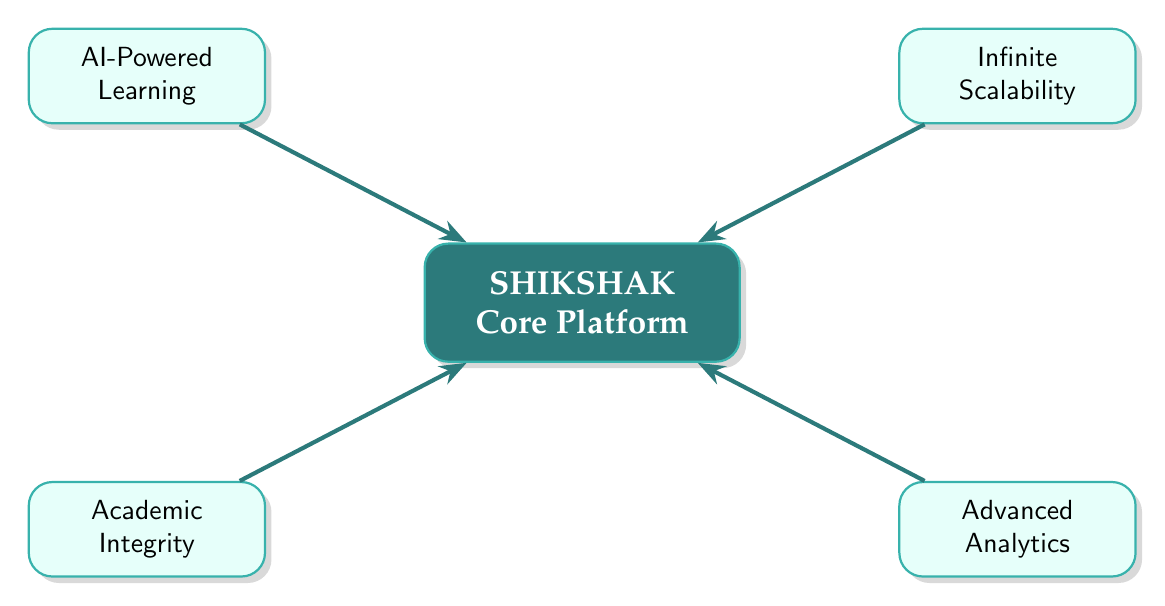
\begin{tikzpicture}[scale=0.9]
    % Central concept
    \node[basic, fill=shikscolPrimary, text=white, minimum width=4cm, minimum height=1.5cm, font=\large\bfseries] 
        (core) at (0,0) {SHIKSHAK\\Core Platform};
    
    % Surrounding pillars
    \node[basic, above left=1.5cm and 2cm of core] (ai) {AI-Powered\\Learning};
    \node[basic, above right=1.5cm and 2cm of core] (scale) {Infinite\\Scalability};
    \node[basic, below left=1.5cm and 2cm of core] (integrity) {Academic\\Integrity};
    \node[basic, below right=1.5cm and 2cm of core] (analytics) {Advanced\\Analytics};
    
    % Connections
    \draw[bigarrow] (ai) -- (core);
    \draw[bigarrow] (scale) -- (core);
    \draw[bigarrow] (integrity) -- (core);
    \draw[bigarrow] (analytics) -- (core);
\end{tikzpicture}
\caption{Core Pillars of the SHIKSHAK Platform}
\end{figure}

\section{The Problem We're Solving}

Modern education faces several critical challenges that demand innovative solutions:

\subsection{Student Engagement Crisis}

Studies show that online course completion rates hover around 5-15\%. Students feel isolated, confused, and unsupported. When they have questions at midnight while studying, they have nowhere to turn except generic search engines that don't understand their specific course context.

\subsection{Academic Integrity}

The shift to remote learning exposed a fundamental weakness: we have no reliable way to verify that students are who they claim to be during assessments, and that they're completing work independently.

\subsection{Teacher Burnout}

Instructors are overwhelmed answering the same questions repeatedly, manually grading assessments, and trying to identify struggling students before it's too late.

\subsection{Infrastructure Limitations}

Traditional LMS platforms struggle when thousands of students attempt to access content simultaneously—especially during exam periods or assignment deadlines.

\section{The Shikshak Solution}

Our platform addresses these challenges through three revolutionary pillars:

\subsection{Intelligent Assistance}

Every student has access to an \textbf{AI Study Companion} that has ingested and understood their entire course material. This isn't a generic chatbot—it's a specialized tutor that can explain complex concepts, provide worked examples, and guide students through problem-solving processes, all while being strictly grounded in the course content to prevent misinformation.

\begin{infobox}[AI Study Companion Features]
\begin{itemize}
    \item 24/7 availability for instant question answering
    \item Context-aware responses based on course material
    \item Step-by-step problem-solving guidance
    \item Multimodal understanding (text, images, code)
    \item Personalized learning recommendations
\end{itemize}
\end{infobox}

\subsection{Verified Integrity}

Our browser-based \textbf{AI Proctoring Suite} uses computer vision to maintain assessment integrity without invasive software installation. It monitors student identity, environment, and behavior patterns in real-time, flagging anomalies for instructor review while respecting privacy by processing most data client-side.

\subsection{Infinite Scalability}

Built on Event-Driven Microservices Architecture, Shikshak can handle 10 students or 100,000 with equal ease. The system automatically scales individual services based on demand, ensuring teachers never have to worry about whether the infrastructure can handle their course enrollment.

\begin{figure}[H]
\centering
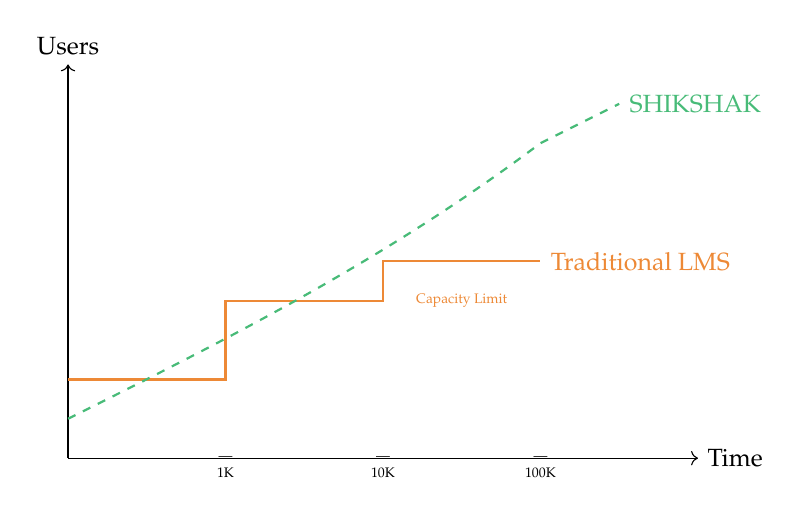
\begin{tikzpicture}
    % Y-axis
    \draw[->] (0,0) -- (0,5) node[above] {\small Users};
    % X-axis
    \draw[->] (0,0) -- (8,0) node[right] {\small Time};
    
    % Traditional LMS (stepped, limited)
    \draw[thick, color=warningOrange] 
        (0,1) -- (2,1) -- (2,2) -- (4,2) -- (4,2.5) -- (6,2.5)
        node[right, font=\small] {Traditional LMS};
    \node[color=warningOrange, font=\tiny] at (5,2) {Capacity Limit};
    
    % SHIKSHAK (smooth scaling)
    \draw[thick, color=successGreen, dashed] 
        (0,0.5) .. controls (2,1.5) and (4,2.5) .. (6,4) -- (7,4.5)
        node[right, font=\small] {SHIKSHAK};
    
    % Annotations
    \node[font=\tiny] at (2,0) {|};
    \node[font=\tiny, below] at (2,0) {1K};
    \node[font=\tiny] at (4,0) {|};
    \node[font=\tiny, below] at (4,0) {10K};
    \node[font=\tiny] at (6,0) {|};
    \node[font=\tiny, below] at (6,0) {100K};
\end{tikzpicture}
\caption{Scalability Comparison: Traditional LMS vs. SHIKSHAK}
\end{figure}

\chapter{Target Audience \& Use Cases}

\section{Higher Education Institutions}

Universities and colleges face increasing pressure to offer robust online and hybrid learning options. Shikshak provides:

\begin{itemize}
    \item \textbf{MOOC-Scale Support:} Handle massive open online courses with thousands of concurrent students, each receiving personalized AI assistance
    \item \textbf{Credible Certifications:} Issue certificates and degrees with confidence, knowing that assessments were completed with verified integrity
    \item \textbf{Analytics for Accreditation:} Comprehensive learning analytics help demonstrate educational outcomes for accreditation bodies
\end{itemize}

\section{Corporate Training Departments}

Enterprises investing in employee development need systems that deliver measurable results:

\begin{itemize}
    \item \textbf{Completion Verification:} Prove that employees actually completed required training modules with proctored assessments
    \item \textbf{Just-In-Time Learning:} AI assistants help employees find specific information within training materials instantly
    \item \textbf{Cost Efficiency:} Reduce dependency on live instructors by automating routine questions and grading
\end{itemize}

\section{Coding Bootcamps \& Professional Development}

Skills-based education providers benefit from:

\begin{itemize}
    \item \textbf{Project-Based Assessment:} Monitor students as they complete real-world projects, ensuring independent work
    \item \textbf{Technical Deep-Dives:} AI can explain complex programming concepts, debug logic errors conceptually, and guide problem-solving
    \item \textbf{Career Credibility:} Employers trust certifications backed by verified assessment integrity
\end{itemize}

\begin{figure}[H]
\centering
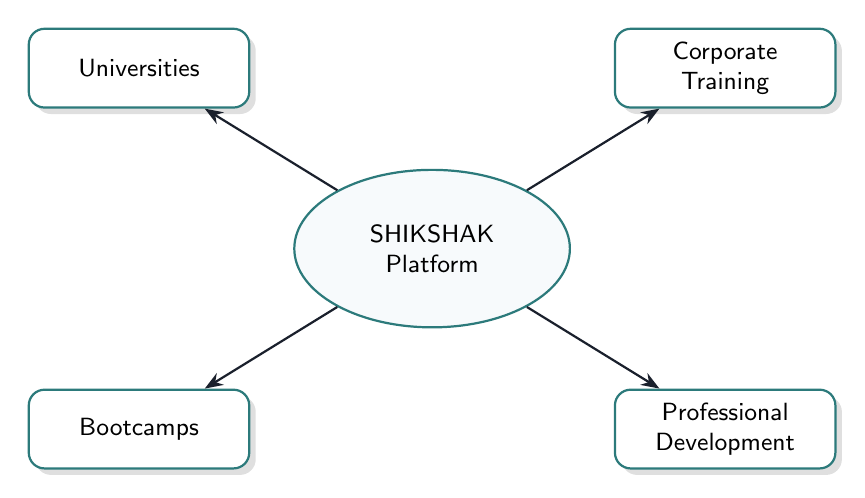
\begin{tikzpicture}[node distance=1.5cm]
    % Central platform
    \node[cloud, minimum width=3.5cm, minimum height=2cm] (platform) {SHIKSHAK\\Platform};
    
    % Use cases around it
    \node[service, above left=of platform] (uni) {Universities};
    \node[service, above right=of platform] (corp) {Corporate\\Training};
    \node[service, below left=of platform] (boot) {Bootcamps};
    \node[service, below right=of platform] (prof) {Professional\\Development};
    
    % Connections
    \foreach \target in {uni, corp, boot, prof} {
        \draw[arrow] (platform) -- (\target);
    }
\end{tikzpicture}
\caption{SHIKSHAK's Diverse Application Domains}
\end{figure}

% PART II: ARCHITECTURE
%\part{System Architecture}

\chapter{Architectural Philosophy}

\section{Microservices-First Design}

Shikshak is built entirely on microservices architecture. This isn't just a trendy buzzword—it's a fundamental architectural choice that provides concrete benefits:

\begin{warningbox}[Key Architectural Principle]
Each service is independently deployable, scalable, and maintainable. This separation of concerns allows teams to work in parallel and scale resources precisely where needed.
\end{warningbox}

\subsection{Benefits of Microservices}

\textbf{Independent Scaling:} The AI RAG service requires significant computational resources and may need 10 server instances during peak hours. Meanwhile, the Authentication service is lightweight and might only need 2 instances. Microservices allow us to scale each component independently based on its specific demands.

\textbf{Technology Flexibility:} Each service can be built with the technology best suited to its purpose. The RAG service might use Python for its rich AI/ML ecosystem, while the Course Service uses Node.js for fast I/O operations. They communicate via standard HTTP and Kafka protocols.

\textbf{Fault Isolation:} If the Payment Service experiences a bug and crashes, students can still watch videos, ask AI questions, and submit assignments. The system degrades gracefully rather than failing catastrophically.

\textbf{Team Autonomy:} Different development teams can own different services, working in parallel without stepping on each other's toes. The Course Service team can deploy updates without coordinating with the RAG Service team.

\begin{figure}[H]
\centering
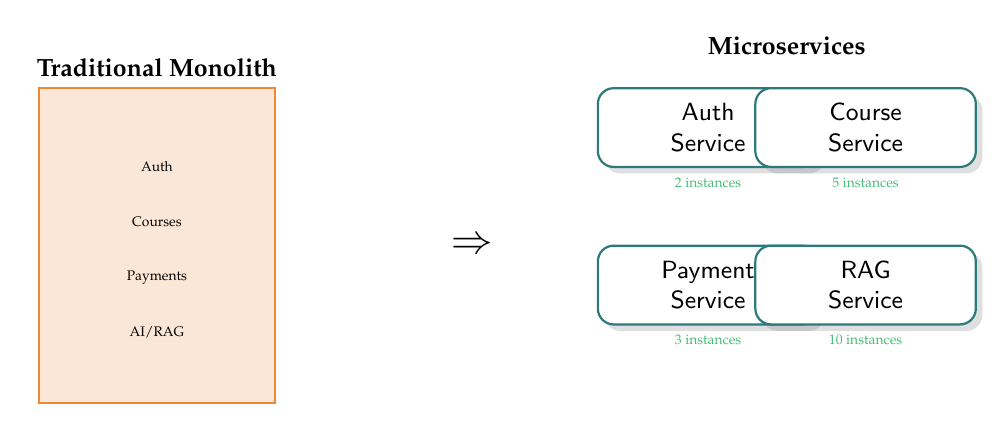
\begin{tikzpicture}[node distance=2cm]
    % Monolith
    \node[draw=warningOrange, fill=warningOrange!20, rectangle, minimum width=3cm, minimum height=4cm, thick] 
        (mono) at (0,0) {};
    \node[above] at (mono.north) {\small\bfseries Traditional Monolith};
    \node[font=\tiny] at (0,1) {Auth};
    \node[font=\tiny] at (0,0.3) {Courses};
    \node[font=\tiny] at (0,-0.4) {Payments};
    \node[font=\tiny] at (0,-1.1) {AI/RAG};
    
    % Arrow
    \node[font=\Large] at (4,0) {$\Rightarrow$};
    
    % Microservices
    \node[service] (auth) at (7,1.5) {Auth\\Service};
    \node[service] (course) at (9,1.5) {Course\\Service};
    \node[service] (payment) at (7,-0.5) {Payment\\Service};
    \node[service] (rag) at (9,-0.5) {RAG\\Service};
    
    \node[above] at (8,2.3) {\small\bfseries Microservices};
    
    % Independent scaling indicators
    \node[font=\tiny, color=successGreen] at (7,0.8) {2 instances};
    \node[font=\tiny, color=successGreen] at (9,0.8) {5 instances};
    \node[font=\tiny, color=successGreen] at (7,-1.2) {3 instances};
    \node[font=\tiny, color=successGreen] at (9,-1.2) {10 instances};
\end{tikzpicture}
\caption{Evolution from Monolithic to Microservices Architecture}
\end{figure}

\section{Event-Driven Communication}

Not all operations need immediate responses. When a teacher uploads a 2GB video file, we don't want them waiting 15 minutes while our servers transcode it into streaming formats. Instead, we use an asynchronous, event-driven approach:

\begin{enumerate}
    \item The upload completes in seconds, and the teacher receives confirmation
    \item An event is published to Apache Kafka: "New video uploaded for Course XYZ"
    \item A background worker service picks up this event and begins processing
    \item When complete, another event triggers: "Video processing complete for Course XYZ"
    \item The Course Service updates the database, and a notification is sent to the teacher
\end{enumerate}

This asynchronous pattern keeps the user interface responsive and allows heavy operations to happen in the background without blocking user interactions.

\begin{figure}[H]
\centering
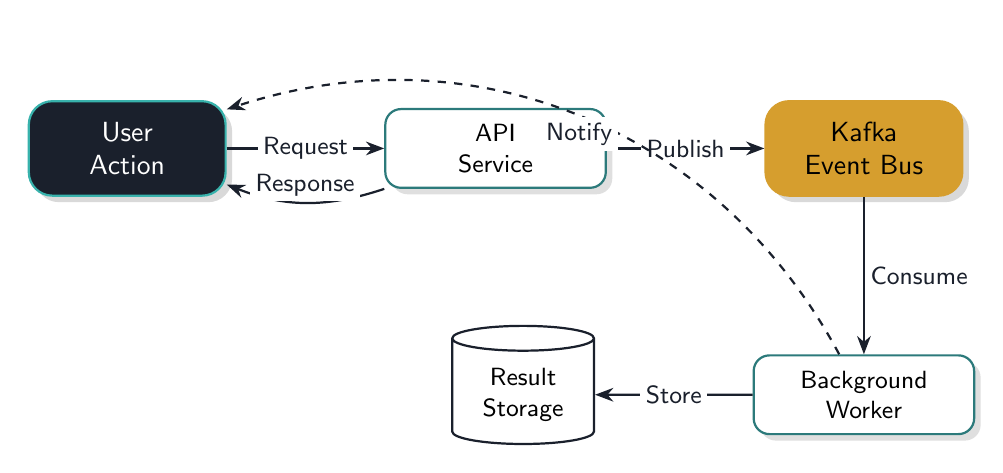
\begin{tikzpicture}[node distance=2.5cm]
    \node[basic, fill=shikscolDark, text=white, minimum width=2.5cm] (user) {User\\Action};
    \node[service, right=2cm of user] (api) {API\\Service};
    \node[basic, fill=shikscolAccent, draw=shikscolAccent, right=2cm of api, minimum width=2.5cm] 
        (kafka) {Kafka\\Event Bus};
    \node[service, below=2cm of kafka] (worker) {Background\\Worker};
    \node[database, left=2cm of worker] (storage) {Result\\Storage};
    
    \draw[arrow] (user) -- node[label] {Request} (api);
    \draw[arrow, bend left=20] (api) to node[label, above] {Response} (user);
    \draw[arrow] (api) -- node[label] {Publish} (kafka);
    \draw[arrow] (kafka) -- node[label, right] {Consume} (worker);
    \draw[arrow] (worker) -- node[label] {Store} (storage);
    \draw[arrow, dashed, bend right=40] (worker) to node[label, below] {Notify} (user);
\end{tikzpicture}
\caption{Event-Driven Asynchronous Processing Pattern}
\end{figure}

\section{Polyglot Persistence}

Different types of data have different storage requirements. Shikshak uses the right database for each job:

\begin{itemize}
    \item \textbf{MongoDB:} Stores hierarchical course structures (Courses $\rightarrow$ Modules $\rightarrow$ Lessons) with flexible schemas that can evolve as educational requirements change
    \item \textbf{Redis:} Serves dual purposes—ultra-fast caching for frequently accessed data, and vector storage for AI embeddings that power semantic search
    \item \textbf{Azure Blob Storage:} Handles large binary files like videos and documents efficiently with CDN integration for global content delivery
\end{itemize}

\begin{figure}[H]
\centering
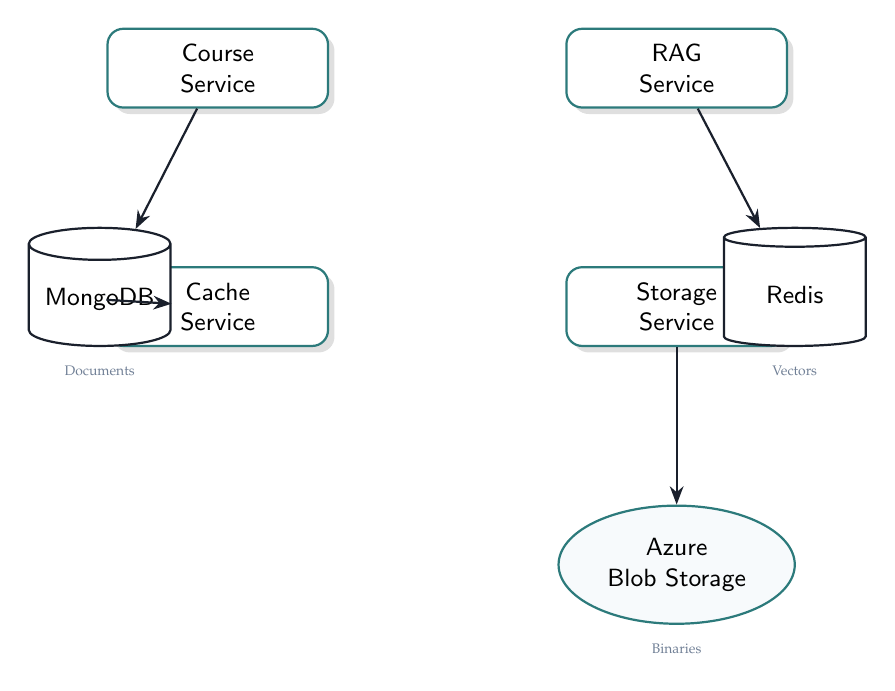
\begin{tikzpicture}[node distance=2.5cm]
    % Central services
    \node[service] (course) {Course\\Service};
    \node[service, right=3cm of course] (rag) {RAG\\Service};
    \node[service, below=2cm of course] (cache) {Cache\\Service};
    \node[service, below=2cm of rag] (storage) {Storage\\Service};
    
    % Databases
    \node[database, below=1.5cm of course, xshift=-1.5cm] (mongo) {MongoDB};
    \node[database, below=1.5cm of rag, xshift=1.5cm] (redis) {Redis};
    \node[cloud, below=2cm of storage, minimum width=3cm] (blob) {Azure\\Blob Storage};
    
    % Connections
    \draw[arrow] (course) -- (mongo);
    \draw[arrow] (rag) -- (redis);
    \draw[arrow] (cache) -- (mongo);
    \draw[arrow] (storage) -- (blob);
    
    % Labels
    \node[font=\tiny, color=shikscolGray] at ([yshift=-0.3cm]mongo.south) {Documents};
    \node[font=\tiny, color=shikscolGray] at ([yshift=-0.3cm]redis.south) {Vectors};
    \node[font=\tiny, color=shikscolGray] at ([yshift=-0.3cm]blob.south) {Binaries};
\end{tikzpicture}
\caption{Polyglot Persistence Strategy}
\end{figure}

\chapter{Core Microservices}

\section{API Gateway Service}

\subsection{Purpose \& Responsibilities}

The Gateway is the front door to our entire backend infrastructure. Every HTTP request from the client must pass through this service. This centralization provides several critical advantages:

\begin{itemize}
    \item \textbf{Security Checkpoint:} SSL certificates are managed here. All HTTPS traffic is decrypted at the gateway, inspected for threats, and then forwarded to internal services over a trusted private network
    \item \textbf{Unified Entry Point:} Clients only need to know one URL. The gateway handles routing requests to the appropriate microservice based on the path
    \item \textbf{Rate Limiting:} Prevents abuse by limiting how many requests a single user can make per minute, protecting backend services from being overwhelmed
    \item \textbf{Request/Response Transformation:} Can modify headers, add authentication tokens, or transform data formats as needed
\end{itemize}

\subsection{Request Flow}

When a student's browser sends a request to view "Course 123, Module 5, Lesson 2", the Gateway:

\begin{enumerate}
    \item Receives the request at: \texttt{/api/v1/courses/123/modules/5/lessons/2}
    \item Validates the JWT token in the request header to confirm the user is logged in
    \item Checks rate limits: Has this user made too many requests recently?
    \item Routes the request to the Course Service's internal address
    \item Receives the response from Course Service
    \item Adds CORS headers if needed for browser compatibility
    \item Returns the response to the client's browser
\end{enumerate}

All of this happens in milliseconds, providing a seamless experience while maintaining security and organization.

\begin{figure}[H]
\centering
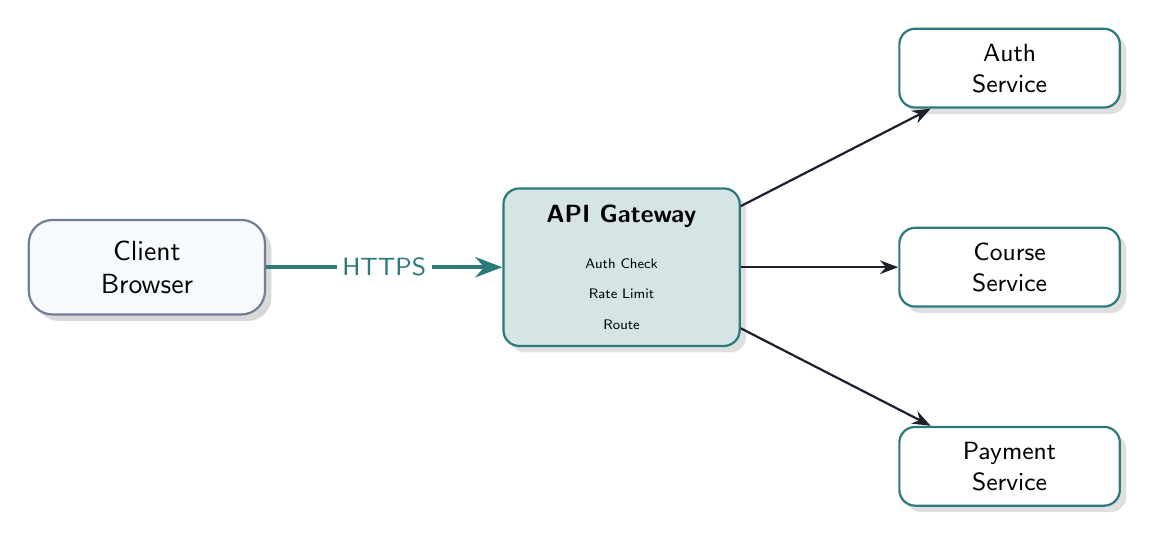
\begin{tikzpicture}[node distance=2cm]
    % Client
    \node[basic, fill=shikscolLight, draw=shikscolGray] (client) {Client\\Browser};
    
    % Gateway
    \node[service, fill=shikscolPrimary!20, right=3cm of client, minimum width=3cm, minimum height=2cm] (gateway) {
        \textbf{API Gateway}\\[0.2cm]
        \tiny Auth Check\\
        \tiny Rate Limit\\
        \tiny Route
    };
    
    % Backend services
    \node[service, above right=1cm and 2cm of gateway] (auth) {Auth\\Service};
    \node[service, right=2cm of gateway] (course) {Course\\Service};
    \node[service, below right=1cm and 2cm of gateway] (payment) {Payment\\Service};
    
    % Arrows
    \draw[bigarrow] (client) -- node[label] {HTTPS} (gateway);
    \draw[arrow] (gateway) -- (auth);
    \draw[arrow] (gateway) -- (course);
    \draw[arrow] (gateway) -- (payment);
\end{tikzpicture}
\caption{API Gateway Request Routing}
\end{figure}

\subsection{Technology Choices}

The Gateway is built with \textbf{Node.js} using the \textbf{Express} framework, chosen for its non-blocking I/O model that allows it to handle thousands of concurrent connections efficiently. It uses minimal CPU because it's primarily forwarding requests rather than processing them.

\section{Authentication Service}

\subsection{The Challenge of Identity}

In educational systems, identity is paramount. We need to answer three questions with certainty:

\begin{itemize}
    \item \textbf{Authentication:} Is this user who they claim to be?
    \item \textbf{Authorization:} What is this user allowed to access?
    \item \textbf{Accountability:} Can we maintain an audit trail of user actions?
\end{itemize}

\subsection{Multi-Strategy Authentication}

Shikshak supports multiple ways for users to prove their identity:

\textbf{OAuth 2.0 Integration:} Users can sign in with Google or GitHub. When they click "Sign in with Google," we redirect them to Google's servers. Google verifies their identity (username, password, two-factor authentication), then sends us back an authorization code confirming their identity. We never see or store their Google password.

\textbf{Email \& Password:} Traditional authentication for users who prefer it. Passwords are hashed using bcrypt with a computational cost factor of 12, meaning even if our database is compromised, the passwords remain computationally infeasible to crack.

\textbf{Magic Links:} For quick access, users can request a one-time login link sent to their verified email address. The link contains a cryptographically secure token valid for 15 minutes.

\begin{figure}[H]
\centering
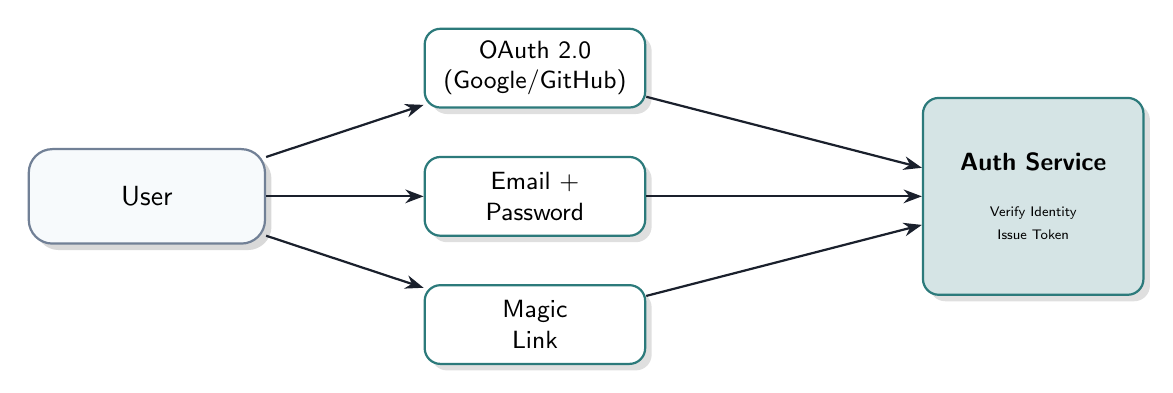
\begin{tikzpicture}[node distance=2.5cm]
    % User
    \node[basic, fill=shikscolLight, draw=shikscolGray] (user) {User};
    
    % Auth methods
    \node[service, above right=0.5cm and 2cm of user] (oauth) {OAuth 2.0\\(Google/GitHub)};
    \node[service, right=2cm of user] (email) {Email +\\Password};
    \node[service, below right=0.5cm and 2cm of user] (magic) {Magic\\Link};
    
    % Auth service
    \node[service, fill=shikscolPrimary!20, right=3.5cm of email, minimum height=2.5cm] 
        (authsvc) {\textbf{Auth Service}\\[0.2cm]\tiny Verify Identity\\[-0.1cm]\tiny Issue Token};
    
    % Arrows
    \draw[arrow] (user) -- (oauth);
    \draw[arrow] (user) -- (email);
    \draw[arrow] (user) -- (magic);
    \draw[arrow] (oauth) -- (authsvc);
    \draw[arrow] (email) -- (authsvc);
    \draw[arrow] (magic) -- (authsvc);
\end{tikzpicture}
\caption{Multi-Strategy Authentication Flow}
\end{figure}

\subsection{Role-Based Access Control}

Not all users are equal. Shikshak defines several roles:

\begin{itemize}
    \item \textbf{Students:} Can view courses they're enrolled in, submit assignments, and take quizzes
    \item \textbf{Teachers:} Can create and modify their own courses, view student progress, and grade assessments
    \item \textbf{Administrators:} Can manage users, configure system settings, and access platform analytics
    \item \textbf{Institution Admins:} Have elevated privileges for their specific organization, managing teachers and students within their institution
\end{itemize}

The Auth Service maintains a mapping of users to roles and enforces these permissions through middleware that intercepts every request.

\subsection{Session Management}

When you log in, the Auth Service creates a session token—a random, cryptographically secure string. This token is stored:

\begin{enumerate}
    \item In the database, associated with your user ID and an expiration timestamp
    \item In your browser as an HTTP-only cookie (JavaScript cannot access it, preventing XSS attacks)
\end{enumerate}

Every subsequent request includes this cookie. The Auth Service validates it by checking if the token exists in the database and hasn't expired. Sessions expire after 7 days of inactivity for security.

\section{Course Management Service}

\subsection{Educational Content Hierarchy}

Online education has a natural structure that Shikshak mirrors in its data model:

\begin{figure}[H]
\centering
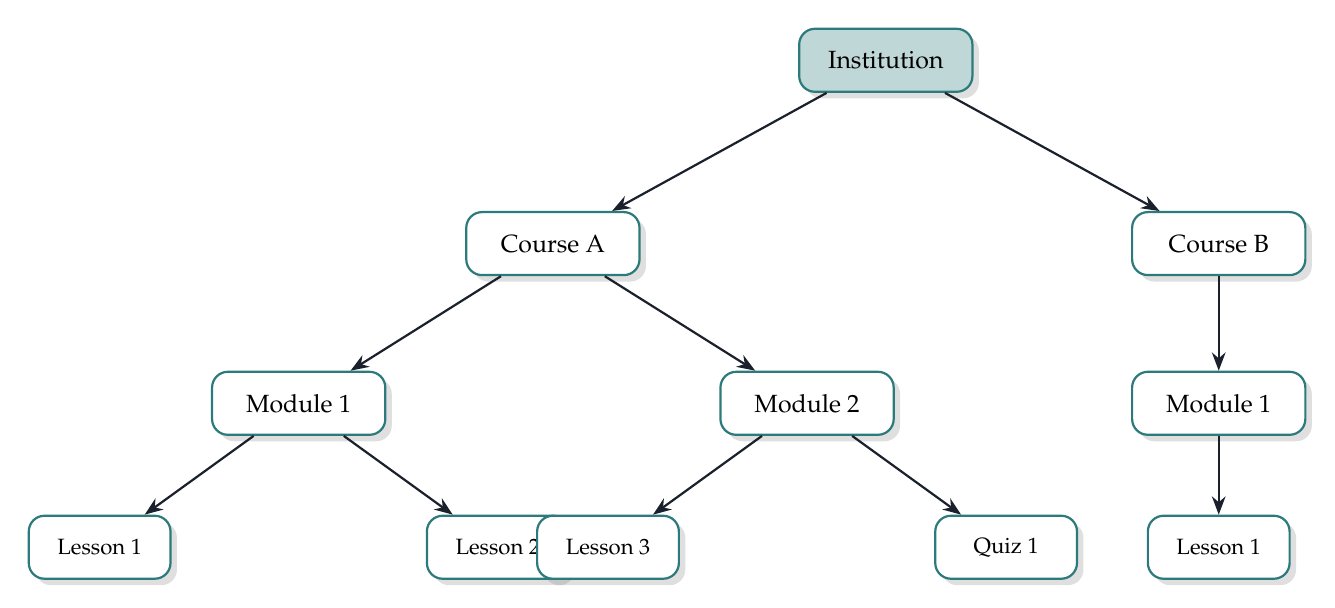
\begin{tikzpicture}[
    node distance=1.2cm and 0.8cm,
    every node/.style={service, minimum width=2.2cm, minimum height=0.8cm, font=\small}
]
    % Top level - Institution
    \node[fill=shikscolPrimary!30] (inst) {Institution};
    
    % Second level - Courses
    \node[below left=1.5cm and 2cm of inst] (courseA) {Course A};
    \node[below right=1.5cm and 2cm of inst] (courseB) {Course B};
    
    % Third level - Modules under Course A
    \node[below left=1.2cm and 1cm of courseA] (mod1a) {Module 1};
    \node[below right=1.2cm and 1cm of courseA] (mod2a) {Module 2};
    
    % Third level - Module under Course B
    \node[below=1.2cm of courseB] (mod1b) {Module 1};
    
    % Fourth level - Lessons under Module 1 (Course A)
    \node[below left=1cm and 0.5cm of mod1a, font=\footnotesize, minimum width=1.8cm] (les1) {Lesson 1};
    \node[below right=1cm and 0.5cm of mod1a, font=\footnotesize, minimum width=1.8cm] (les2) {Lesson 2};
    
    % Fourth level - Lessons under Module 2 (Course A)
    \node[below left=1cm and 0.5cm of mod2a, font=\footnotesize, minimum width=1.8cm] (les3) {Lesson 3};
    \node[below right=1cm and 0.5cm of mod2a, font=\footnotesize, minimum width=1.8cm] (quiz1) {Quiz 1};
    
    % Fourth level - Lesson under Module 1 (Course B)
    \node[below=1cm of mod1b, font=\footnotesize, minimum width=1.8cm] (les1b) {Lesson 1};
    
    % Connections
    \draw[arrow] (inst) -- (courseA);
    \draw[arrow] (inst) -- (courseB);
    \draw[arrow] (courseA) -- (mod1a);
    \draw[arrow] (courseA) -- (mod2a);
    \draw[arrow] (courseB) -- (mod1b);
    \draw[arrow] (mod1a) -- (les1);
    \draw[arrow] (mod1a) -- (les2);
    \draw[arrow] (mod2a) -- (les3);
    \draw[arrow] (mod2a) -- (quiz1);
    \draw[arrow] (mod1b) -- (les1b);
\end{tikzpicture}
\caption{Educational Content Hierarchy}
\end{figure}

\textbf{Institution Level:} A university or company running the platform.

\textbf{Course Level:} An individual class, like "Introduction to Machine Learning" or "Corporate Ethics Training."

\textbf{Module Level:} Major topics within a course, such as "Neural Networks" or "Decision Trees."

\textbf{Lesson Level:} Individual learning units, typically a video lecture, reading, or interactive activity.

\textbf{Assessment Level:} Quizzes, exams, and assignments that test understanding.

The Course Service manages this entire hierarchy, tracking relationships and permissions.

\subsection{Content Delivery}

When a student clicks to watch a video lesson, the Course Service:

\begin{enumerate}
    \item Verifies the student is enrolled in the course (authorization check)
    \item Checks if any prerequisite lessons must be completed first
    \item Retrieves the video URL from cloud storage
    \item Generates a time-limited, signed URL valid for 2 hours (prevents sharing links)
    \item Logs that the student accessed this lesson (for progress tracking)
    \item Returns the URL along with metadata (title, description, duration, transcript)
\end{enumerate}

\subsection{Progress Tracking}

The service maintains detailed records of student progress:

\begin{itemize}
    \item Which lessons have been viewed and what percentage was watched
    \item Quiz scores and attempt timestamps
    \item Assignment submission status
    \item Time spent on each lesson (captured via heartbeat pings from the video player)
    \item Completion status for modules and overall course
\end{itemize}

Teachers can access these analytics to identify struggling students and adapt their teaching strategy.

\begin{infobox}[Progress Metrics]
The Course Service tracks over 20 different engagement metrics per student, including:
\begin{itemize}
    \item Video completion rates
    \item Quiz attempt patterns
    \item Time-on-task measurements
    \item Discussion forum participation
    \item Assignment submission timeliness
\end{itemize}
\end{infobox}

\subsection{Dynamic Content Rendering}

Course content isn't static. Teachers can:

\begin{itemize}
    \item Reorder modules and lessons by dragging them in the UI
    \item Hide lessons until a specific date (for phased content release)
    \item Update lesson content and have changes reflect immediately for all students
    \item Attach supplementary materials (PDFs, slides, external links)
\end{itemize}

The Course Service handles all this complexity while maintaining performance even with thousands of students accessing content simultaneously.

\section{RAG (Retrieval-Augmented Generation) Service}

\subsection{The AI Brain of Shikshak}

This is perhaps the most technically sophisticated service in the entire platform. It's what enables students to ask natural language questions and receive accurate, context-aware answers grounded in their course material.

\subsection{Understanding Vector Embeddings}

Computers don't understand language the way humans do. They work with numbers. Vector embeddings are a way to convert text into high-dimensional numerical coordinates that capture semantic meaning.

For example, the sentence "The cat sat on the mat" might become a vector like:
\begin{center}
\texttt{[0.23, -0.45, 0.89, ..., 0.12]}
\end{center}
(with typically 768 or 1536 dimensions).

Similar meanings produce similar vectors. "The feline rested on the rug" would have a vector mathematically close to the first one, even though the exact words are different. This allows us to search by meaning rather than just keyword matching.

\begin{figure}[H]
\centering
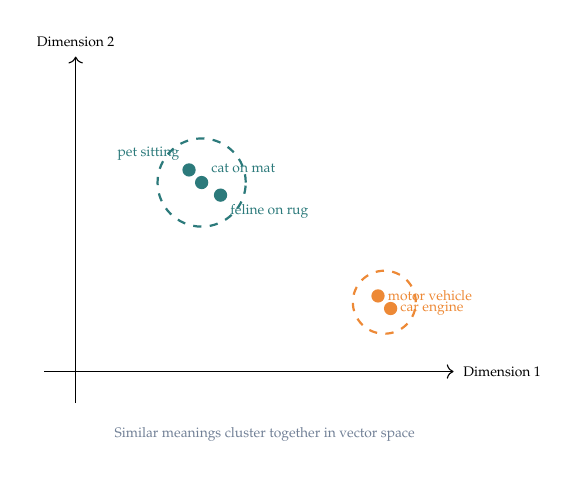
\begin{tikzpicture}[scale=0.8]
    % 2D representation of vector space
    \draw[->] (-0.5,0) -- (6,0) node[right] {\tiny Dimension 1};
    \draw[->] (0,-0.5) -- (0,5) node[above] {\tiny Dimension 2};
    
    % Similar concepts clustered
    \fill[shikscolPrimary] (2,3) circle (3pt) node[above right, font=\tiny] {cat on mat};
    \fill[shikscolPrimary] (2.3,2.8) circle (3pt) node[below right, font=\tiny] {feline on rug};
    \fill[shikscolPrimary] (1.8,3.2) circle (3pt) node[above left, font=\tiny] {pet sitting};
    
    % Different concept
    \fill[warningOrange] (5,1) circle (3pt) node[right, font=\tiny] {car engine};
    \fill[warningOrange] (4.8,1.2) circle (3pt) node[right, font=\tiny] {motor vehicle};
    
    % Circles showing clusters
    \draw[shikscolPrimary, dashed, thick] (2,3) circle (0.7cm);
    \draw[warningOrange, dashed, thick] (4.9,1.1) circle (0.5cm);
    
    \node[font=\tiny, color=shikscolGray] at (3,-1) {Similar meanings cluster together in vector space};
\end{tikzpicture}
\caption{Conceptual Visualization of Vector Embeddings}
\end{figure}

\subsection{The Indexing Process}

When a teacher uploads course material (video transcripts, lecture notes, textbook chapters), the RAG Service:

\begin{enumerate}
    \item \textbf{Chunks the Content:} Breaks large documents into manageable pieces (typically 500-1000 words each with 100-word overlap to maintain context across boundaries)
    \item \textbf{Generates Embeddings:} Each chunk is sent to an embedding model that converts the text into a vector. Shikshak uses OpenAI's text-embedding-ada-002 model or Azure's equivalent
    \item \textbf{Stores in Vector Database:} The vectors are stored in Redis with its vector search capabilities, indexed for fast similarity lookups
    \item \textbf{Maintains Metadata:} Each vector is tagged with metadata: which course it belongs to, what module, lesson, page number, etc.
\end{enumerate}

\subsection{The Query Process}

When a student asks \textit{"How does gradient descent work in backpropagation?"}, the RAG Service:

\begin{enumerate}
    \item \textbf{Vectorizes the Question:} The question is converted into a vector using the same embedding model
    \item \textbf{Searches for Similar Content:} Redis performs a cosine similarity search, finding the top 5-10 chunks from the course material that are most semantically similar to the question vector
    \item \textbf{Constructs a Prompt:} The retrieved chunks are assembled into a prompt for the LLM
    \item \textbf{Generates Response:} The prompt is sent to Azure OpenAI (GPT-4) which generates a comprehensive answer grounded in the provided material
    \item \textbf{Returns with Citations:} The answer is sent back to the student, often with references to specific lessons where they can learn more
\end{enumerate}

This entire process completes in 2-4 seconds, providing students with instant, accurate assistance 24/7.

\begin{figure}[H]
\centering
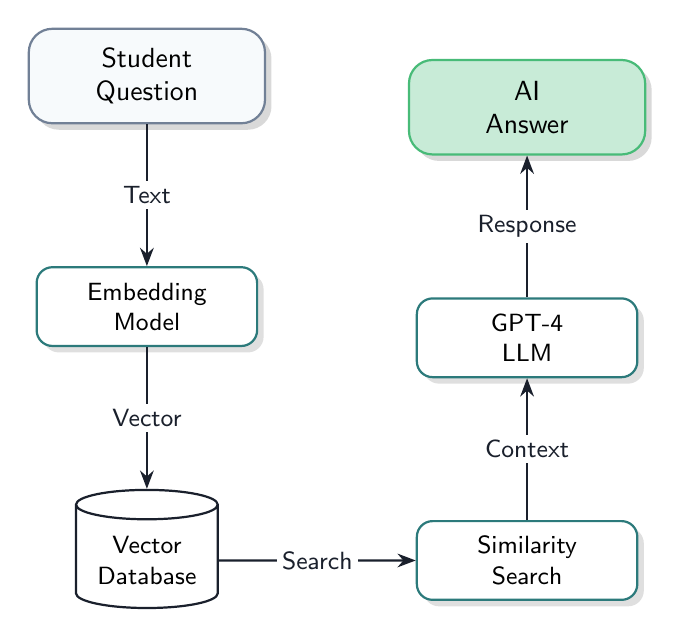
\begin{tikzpicture}[node distance=1.8cm]
    \node[basic, fill=shikscolLight, draw=shikscolGray, minimum width=3cm] (student) {Student\\Question};
    \node[service, below=of student] (embed1) {Embedding\\Model};
    \node[database, below=of embed1] (vector) {Vector\\Database};
    \node[service, right=2.5cm of vector] (retrieve) {Similarity\\Search};
    \node[service, above=of retrieve] (llm) {GPT-4\\LLM};
    \node[basic, fill=successGreen!30, draw=successGreen, above=of llm, minimum width=3cm] 
        (answer) {AI\\Answer};
    
    \draw[arrow] (student) -- node[label] {Text} (embed1);
    \draw[arrow] (embed1) -- node[label] {Vector} (vector);
    \draw[arrow] (vector) -- node[label] {Search} (retrieve);
    \draw[arrow] (retrieve) -- node[label] {Context} (llm);
    \draw[arrow] (llm) -- node[label] {Response} (answer);
\end{tikzpicture}
\caption{RAG Service Query Flow}
\end{figure}

\subsection{Preventing Hallucinations}

One of the biggest challenges with AI is "hallucination"—when models generate false information confidently. The RAG approach mitigates this by:

\begin{itemize}
    \item Constraining the AI to only answer based on provided course material
    \item Including explicit instructions to admit when it doesn't know something
    \item Showing students which course sections the answer was derived from
    \item Allowing teachers to review and override AI responses
\end{itemize}

\begin{warningbox}[Quality Control]
All AI-generated responses include confidence scores and source citations. Teachers can flag incorrect responses, which are used to continuously improve the system through fine-tuning and prompt engineering.
\end{warningbox}

\section{Payment Service}

\subsection{Transactional Integrity}

Handling payments in an educational platform requires absolute reliability. Students must never be charged twice, and teachers must always receive credit for their course sales. The Payment Service ensures this through careful transaction management.

\subsection{The Purchase Flow}

When a student clicks "Enroll" on a paid course:

\begin{enumerate}
    \item \textbf{Price Verification:} The service confirms the current price (in case the teacher changed it since the student opened the page)
    \item \textbf{Duplicate Check:} Verifies the student hasn't already purchased this course
    \item \textbf{Payment Gateway:} Creates a checkout session with Stripe or equivalent, generating a secure payment page
    \item \textbf{Webhook Handling:} When Stripe confirms payment, a webhook notifies our Payment Service immediately
    \item \textbf{Database Update:} The student is marked as enrolled in the course atomically (either the entire operation succeeds or none of it does)
    \item \textbf{Event Publication:} A Kafka event announces "Student X enrolled in Course Y" so other services can react (send welcome email, update analytics, etc.)
\end{enumerate}

\begin{figure}[H]
\centering
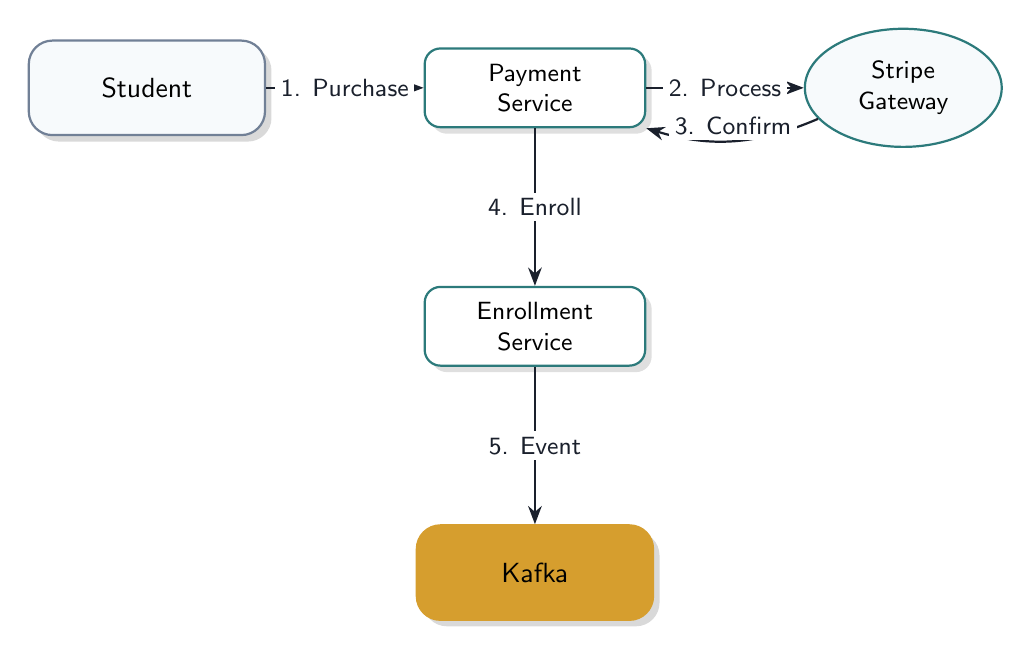
\begin{tikzpicture}[node distance=2cm]
    \node[basic, fill=shikscolLight, draw=shikscolGray] (student) {Student};
    \node[service, right=of student] (payment) {Payment\\Service};
    \node[cloud, minimum width=2.5cm, right=of payment] (stripe) {Stripe\\Gateway};
    \node[service, below=of payment] (enroll) {Enrollment\\Service};
    \node[basic, fill=shikscolAccent, draw=shikscolAccent, below=of enroll] (kafka) {Kafka};
    
    \draw[arrow] (student) -- node[label] {1. Purchase} (payment);
    \draw[arrow] (payment) -- node[label] {2. Process} (stripe);
    \draw[arrow, bend left=20] (stripe) to node[label, above] {3. Confirm} (payment);
    \draw[arrow] (payment) -- node[label] {4. Enroll} (enroll);
    \draw[arrow] (enroll) -- node[label] {5. Event} (kafka);
\end{tikzpicture}
\caption{Secure Payment Processing Flow}
\end{figure}

\subsection{Revenue Distribution}

For marketplace-style deployments where multiple teachers sell courses on a shared platform, the Payment Service handles complex revenue splitting:

\begin{itemize}
    \item Platform fee (e.g., 20\% to Shikshak operators)
    \item Teacher commission (e.g., 75\% to course creator)
    \item Affiliate commission (e.g., 5\% to the blog that referred the student)
\end{itemize}

This is all configured per course and calculated automatically at purchase time.

\section{Notification Service}

\subsection{Keeping Users Informed}

An LMS is ineffective if students miss important updates. The Notification Service ensures timely, relevant communication across multiple channels.

\subsection{Notification Types}

\textbf{Email Notifications:} Sent for major events like course enrollment confirmation, assignment grading, or deadline reminders. Uses SendGrid or AWS SES for reliable delivery with bounce handling.

\textbf{In-App Notifications:} Displayed in the web interface with a bell icon counter. Students see these immediately when logged in.

\textbf{Push Notifications:} For the mobile app (future feature), delivered via Firebase Cloud Messaging.

\begin{figure}[H]
\centering
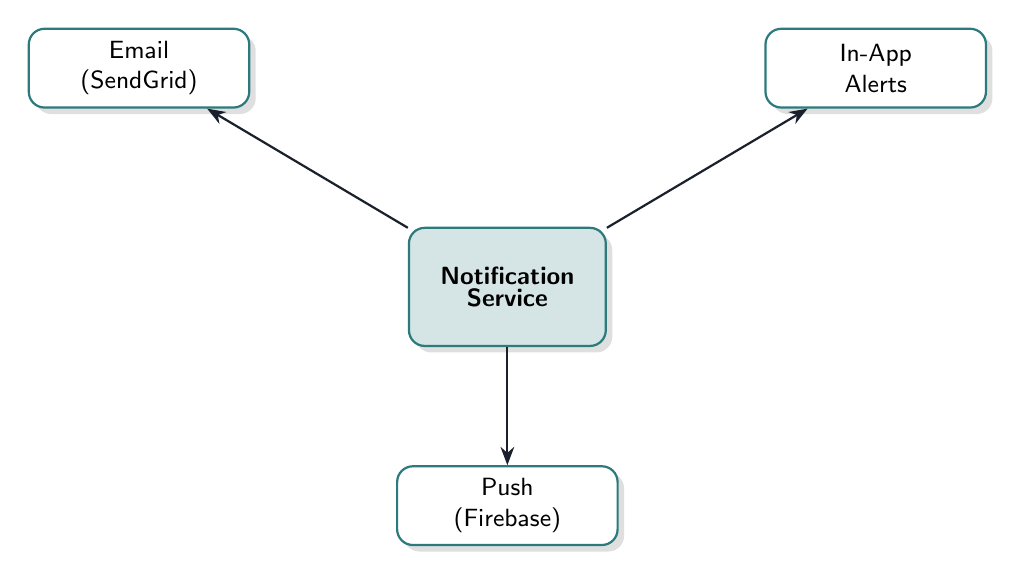
\begin{tikzpicture}[node distance=2.5cm]
    % Central notification service
    \node[service, fill=shikscolPrimary!20, minimum width=2.5cm, minimum height=1.5cm] 
        (notif) {\textbf{Notification}\\[-0.1cm]\textbf{Service}};
    
    % Channels
    \node[service, above left=1.5cm and 2cm of notif] (email) {Email\\(SendGrid)};
    \node[service, above right=1.5cm and 2cm of notif] (app) {In-App\\Alerts};
    \node[service, below=1.5cm of notif] (push) {Push\\(Firebase)};
    
    % Arrows from service to channels
    \draw[arrow] (notif) -- (email);
    \draw[arrow] (notif) -- (app);
    \draw[arrow] (notif) -- (push);
\end{tikzpicture}
\caption{Multi-Channel Notification System}
\end{figure}

\subsection{Smart Batching}

Instead of sending 50 separate emails if a teacher posts 50 new announcements, the Notification Service batches them into a single daily digest email, reducing inbox overload while ensuring students stay informed.

\subsection{Preference Management}

Students can customize which notifications they receive, opting out of non-essential updates while still receiving critical information like grade releases and deadline reminders.

\chapter{Technology Stack Deep Dive}

\section{Frontend: Next.js Framework}

\subsection{Why Next.js}

Shikshak's frontend is built with \textbf{Next.js 15}, a React-based framework that provides several critical advantages for an LMS:

\begin{itemize}
    \item \textbf{Server-Side Rendering (SSR):} When a student clicks a link to a course, the server pre-renders the HTML with all the course information before sending it to the browser. This provides instant content visibility and excellent SEO
    \item \textbf{Static Site Generation (SSG):} For content that doesn't change often (like the marketing homepage), Next.js can generate HTML at build time, serving it with blazing speed from a CDN
    \item \textbf{App Router:} The latest Next.js architecture organizes code by feature, making large applications more maintainable
    \item \textbf{Image Optimization:} Automatically resizes and optimizes course thumbnails and profile pictures
\end{itemize}

\subsection{State Management with Zustand}

While Next.js handles server state beautifully, client-side state (like "is the video player currently playing" or "what's the user's selected theme") requires dedicated management. Shikshak uses \textbf{Zustand}, a lightweight state library that's simpler than Redux but more powerful than React's built-in Context API.

\subsection{Styling with Tailwind CSS}

Every UI component is styled using \textbf{Tailwind CSS 4's} utility-first approach. Instead of writing custom CSS classes, developers apply pre-built classes directly in the HTML. This ensures design consistency and speeds up development significantly.

\section{Backend: Node.js Ecosystem}

\subsection{Non-Blocking I/O}

Most LMS operations are I/O-bound rather than CPU-bound. When fetching data from a database or calling an external API, the server spends most of its time waiting for responses. Node.js handles this brilliantly with its event loop architecture.

Traditional threaded servers create a new thread for each request, which consumes memory. Node.js uses a single thread with asynchronous callbacks, allowing thousands of concurrent connections with minimal resource usage.

\begin{figure}[H]
\centering
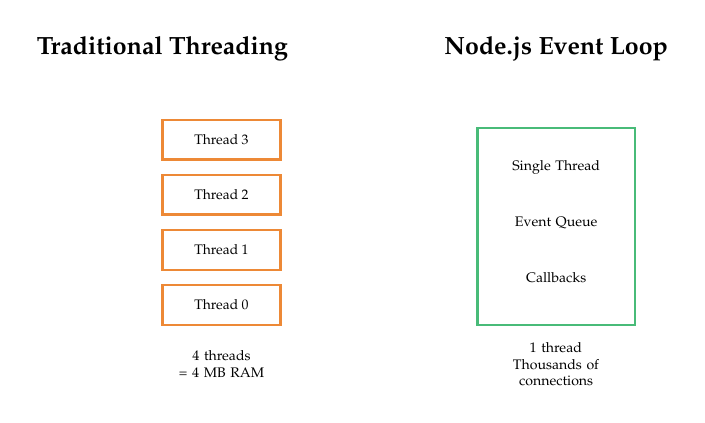
\begin{tikzpicture}
    % Traditional threading
    \node[font=\small\bfseries] at (0,3.5) {Traditional Threading};
    \foreach \i in {0,1,2,3} {
        \draw[thick, warningOrange] (0,\i*0.7) rectangle (1.5,\i*0.7+0.5);
        \node[font=\tiny] at (0.75,\i*0.7+0.25) {Thread \i};
    }
    \node[font=\tiny, text width=2cm, align=center] at (0.75,-0.5) 
        {4 threads\\= 4 MB RAM};
    
    % Node.js event loop
    \node[font=\small\bfseries] at (5,3.5) {Node.js Event Loop};
    \draw[thick, successGreen] (4,0) rectangle (6,2.5);
    \node[font=\tiny, text width=1.5cm, align=center] at (5,2) {Single Thread};
    \node[font=\tiny, text width=1.5cm, align=center] at (5,1.3) {Event Queue};
    \node[font=\tiny, text width=1.5cm, align=center] at (5,0.6) {Callbacks};
    \node[font=\tiny, text width=2cm, align=center] at (5,-0.5) 
        {1 thread\\Thousands of\\connections};
\end{tikzpicture}
\caption{Threading Model Comparison}
\end{figure}

\subsection{npm Package Ecosystem}

Node.js has the world's largest package registry. Need JWT authentication? Install \texttt{jsonwebtoken}. Need to resize images? Install \texttt{sharp}. This rich ecosystem allows rapid development without reinventing wheels.

\section{Database: MongoDB}

\subsection{Document-Oriented Schema}

Educational content is hierarchical and variable in structure. A Biology course might have lab videos, while a Mathematics course has interactive problem sets. MongoDB's flexible document schema adapts perfectly.

\subsection{Horizontal Scaling with Sharding}

When Shikshak grows to millions of users, a single database server won't suffice. MongoDB supports sharding—splitting data across multiple servers based on a shard key (like user ID or course ID). Queries automatically route to the correct shard, distributing load.

\begin{figure}[H]
\centering
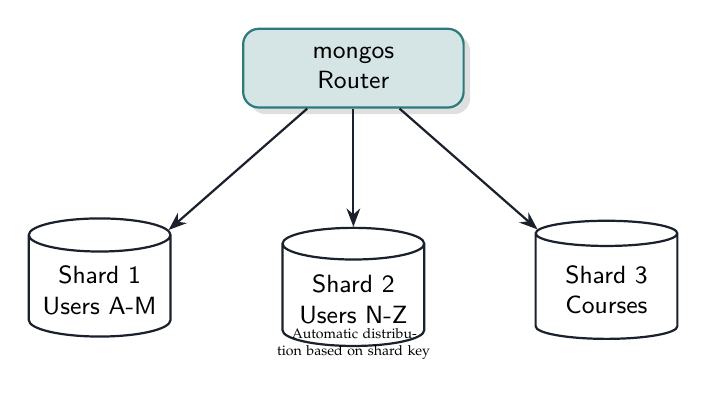
\begin{tikzpicture}[node distance=2cm]
    % Query router
    \node[service, fill=shikscolPrimary!20] (router) {mongos\\Router};
    
    % Shards
    \node[database, below left=1.5cm and 1cm of router] (shard1) {Shard 1\\Users A-M};
    \node[database, below=1.5cm of router] (shard2) {Shard 2\\Users N-Z};
    \node[database, below right=1.5cm and 1cm of router] (shard3) {Shard 3\\Courses};
    
    % Connections
    \draw[arrow] (router) -- (shard1);
    \draw[arrow] (router) -- (shard2);
    \draw[arrow] (router) -- (shard3);
    
    \node[font=\tiny, text width=3cm, align=center] at (0,-3.5) 
        {Automatic distribution based on shard key};
\end{tikzpicture}
\caption{MongoDB Sharding Architecture}
\end{figure}

\subsection{Replica Sets for High Availability}

Every production MongoDB deployment runs with replica sets: one primary server handles writes, while multiple secondary servers replicate data in real-time. If the primary fails, a secondary automatically promotes itself to primary within seconds, ensuring near-zero downtime.

\section{Message Queue: Apache Kafka}

\subsection{What Makes Kafka Special}

Kafka isn't just a message queue—it's a distributed streaming platform built for massive scale. While traditional queues like RabbitMQ work well for moderate loads, Kafka can handle millions of events per second.

\subsection{Topics and Partitions}

Kafka organizes events into topics. Shikshak might have topics like:

\begin{itemize}
    \item \texttt{user.registered} - New user signups
    \item \texttt{video.uploaded} - New course videos
    \item \texttt{assessment.submitted} - Student quiz/exam submissions
    \item \texttt{payment.completed} - Successful course purchases
\end{itemize}

Each topic is further divided into partitions for parallel processing. If video processing workers need to handle high load, they can consume from multiple partitions simultaneously.

\begin{figure}[H]
\centering
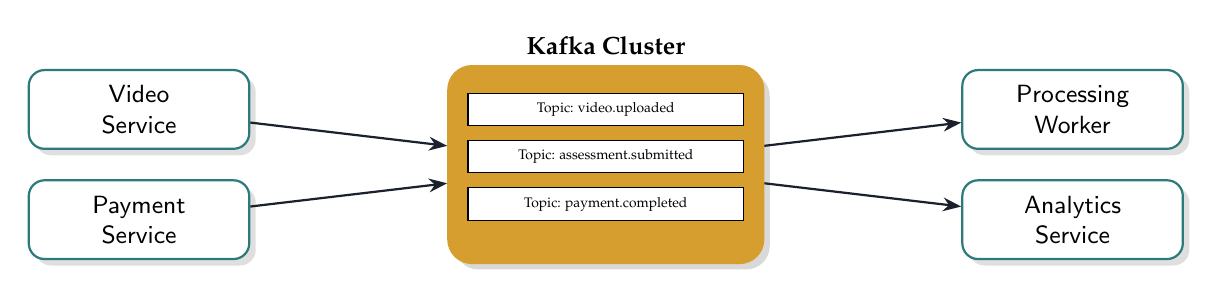
\begin{tikzpicture}[node distance=1.5cm]
    % Kafka cluster
    \node[basic, fill=shikscolAccent, draw=shikscolAccent, minimum width=4cm, minimum height=2.5cm] 
        (kafka) at (0,0) {};
    \node[above] at (kafka.north) {\small\bfseries Kafka Cluster};
    
    % Topics
    \node[font=\tiny, fill=white, draw, minimum width=3.5cm] at (0,0.7) 
        {Topic: video.uploaded};
    \node[font=\tiny, fill=white, draw, minimum width=3.5cm] at (0,0.1) 
        {Topic: assessment.submitted};
    \node[font=\tiny, fill=white, draw, minimum width=3.5cm] at (0,-0.5) 
        {Topic: payment.completed};
    
    % Producers
    \node[service, left=2.5cm of kafka, yshift=0.7cm] (prod1) {Video\\Service};
    \node[service, left=2.5cm of kafka, yshift=-0.7cm] (prod2) {Payment\\Service};
    
    % Consumers
    \node[service, right=2.5cm of kafka, yshift=0.7cm] (cons1) {Processing\\Worker};
    \node[service, right=2.5cm of kafka, yshift=-0.7cm] (cons2) {Analytics\\Service};
    
    % Arrows
    \draw[arrow] (prod1) -- (kafka);
    \draw[arrow] (prod2) -- (kafka);
    \draw[arrow] (kafka) -- (cons1);
    \draw[arrow] (kafka) -- (cons2);
\end{tikzpicture}
\caption{Kafka Event Streaming Architecture}
\end{figure}

\subsection{Event Replay}

Unlike traditional queues that delete messages after consumption, Kafka retains events for a configured period (e.g., 7 days). This allows:

\begin{itemize}
    \item \textbf{Debugging:} If a bug caused incorrect processing last week, we can replay those events through a fixed version of the code
    \item \textbf{Analytics:} A new analytics service can read historical events to build dashboards retroactively
    \item \textbf{Disaster Recovery:} If a database is corrupted, we can rebuild it by replaying all events in order
\end{itemize}

\section{Caching \& Vector Storage: Redis}

\subsection{Microsecond Latency}

Redis stores data entirely in RAM, providing sub-millisecond response times. This makes it perfect for:

\begin{itemize}
    \item \textbf{Session Storage:} User session tokens are stored in Redis for instant authentication checks
    \item \textbf{Leaderboard Caching:} Course leaderboards showing top-performing students are cached for 5 minutes rather than recalculating from the database on every page load
    \item \textbf{Rate Limiting:} Track how many API requests each user has made in the last minute, enforcing limits without database overhead
\end{itemize}

\subsection{Vector Search Capabilities}

Recent Redis versions include RedisSearch with vector similarity searching. This allows the RAG service to store and query millions of embedding vectors efficiently without requiring a specialized vector database like Pinecone or Weaviate.

\section{Cloud Infrastructure: Azure}

\subsection{Blob Storage}

All video files, PDFs, and user-uploaded content live in \textbf{Azure Blob Storage}. Benefits include:

\begin{itemize}
    \item \textbf{Scalability:} Store petabytes of data without managing disk arrays
    \item \textbf{CDN Integration:} Integrate with Azure CDN for global content delivery with servers near students worldwide
    \item \textbf{Lifecycle Policies:} Automatically move old content to cheaper "cool" or "archive" tiers
\end{itemize}

\subsection{OpenAI Service}

Azure's OpenAI deployment provides enterprise-grade access to GPT-4 with guaranteed uptime SLAs, data residency compliance, and usage quotas that ensure consistent RAG service performance.

\begin{figure}[H]
\centering
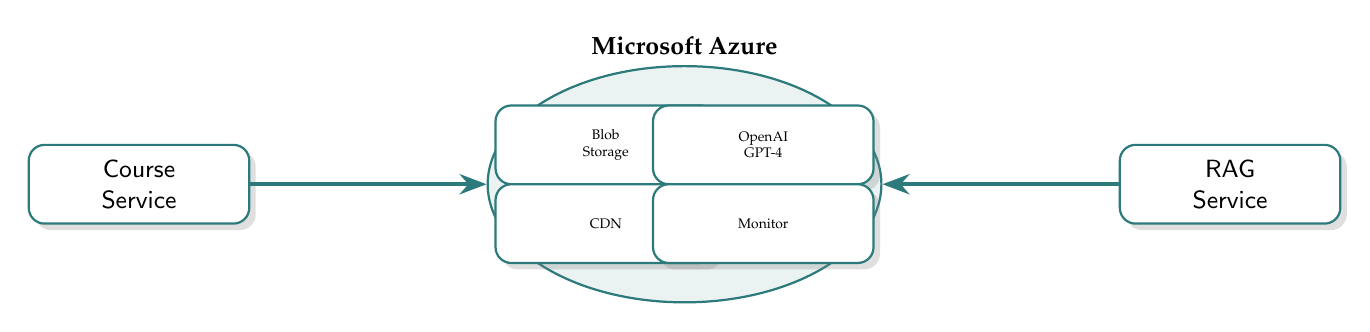
\begin{tikzpicture}[node distance=2.5cm]
    % Azure cloud
    \node[cloud, minimum width=5cm, minimum height=3cm, fill=shikscolPrimary!10] (azure) at (0,0) {};
    \node[above, font=\small\bfseries] at (azure.north) {Microsoft Azure};
    
    % Services inside
    \node[service, font=\tiny] at (-1,0.5) {Blob\\Storage};
    \node[service, font=\tiny] at (1,0.5) {OpenAI\\GPT-4};
    \node[service, font=\tiny] at (-1,-0.5) {CDN};
    \node[service, font=\tiny] at (1,-0.5) {Monitor};
    
    % SHIKSHAK services connecting
    \node[service, left=3cm of azure] (course) {Course\\Service};
    \node[service, right=3cm of azure] (rag) {RAG\\Service};
    
    \draw[bigarrow] (course) -- (azure);
    \draw[bigarrow] (rag) -- (azure);
\end{tikzpicture}
\caption{Azure Cloud Services Integration}
\end{figure}

\chapter{Advanced Features}

\section{AI Proctoring System}

\subsection{The Challenge of Remote Assessment Integrity}

Traditional in-person exams provide natural safeguards: an instructor watches students, controls the environment, and verifies identities. Remote exams lack these controls, creating opportunities for cheating. Shikshak's AI Proctoring System restores integrity while respecting student privacy.

\subsection{Face Verification}

Before an exam begins, students complete an enrollment process:

\begin{enumerate}
    \item \textbf{ID Capture:} Student uploads a photo of their government ID
    \item \textbf{Live Photo:} Student takes a selfie using their webcam
    \item \textbf{Face Encoding:} Our system (using MediaPipe's Face Detection) creates a mathematical representation of facial features—not storing the actual photo to protect privacy
\end{enumerate}

During the exam:

\begin{enumerate}
    \item Webcam captures periodic snapshots (every 60 seconds)
    \item Faces are detected and encoded client-side (in the browser)
    \item Encodings are compared to the enrolled face
    \item If no face is detected or a different person appears, an alert is flagged for instructor review
\end{enumerate}

\begin{figure}[H]
\centering
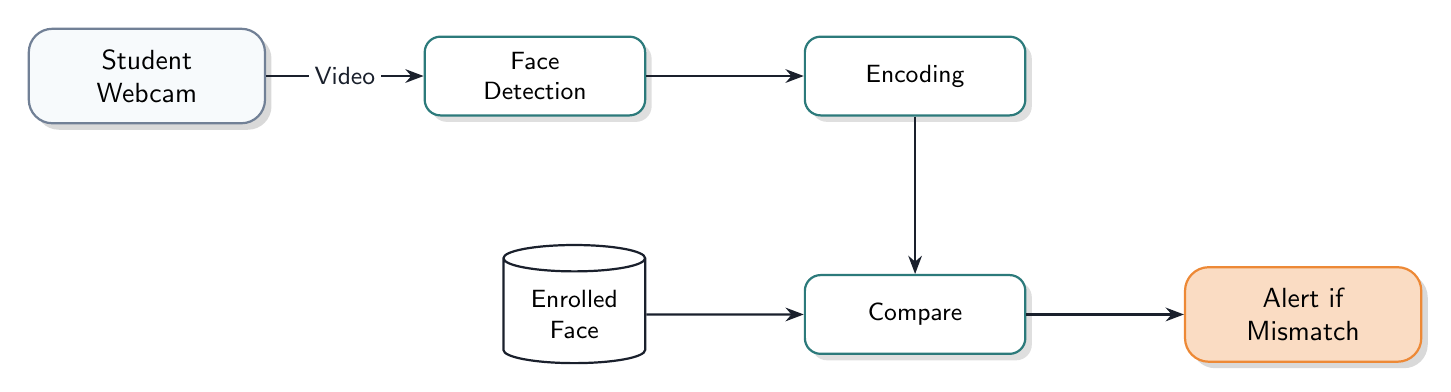
\begin{tikzpicture}[node distance=2cm]
    % Student
    \node[basic, fill=shikscolLight, draw=shikscolGray] (student) {Student\\Webcam};
    
    % Processing steps
    \node[service, right=of student] (detect) {Face\\Detection};
    \node[service, right=of detect] (encode) {Encoding};
    \node[service, below=of encode] (compare) {Compare};
    \node[database, left=of compare] (enrolled) {Enrolled\\Face};
    
    % Alert
    \node[basic, fill=warningOrange!30, draw=warningOrange, right=of compare] 
        (alert) {Alert if\\Mismatch};
    
    % Arrows
    \draw[arrow] (student) -- node[label] {Video} (detect);
    \draw[arrow] (detect) -- (encode);
    \draw[arrow] (encode) -- (compare);
    \draw[arrow] (enrolled) -- (compare);
    \draw[arrow] (compare) -- (alert);
\end{tikzpicture}
\caption{Face Verification Pipeline}
\end{figure}

\subsection{Gaze Tracking}

Students looking away from the screen for extended periods may be reading notes or using a second device. The system tracks:

\begin{itemize}
    \item Eye position relative to screen (using pupil detection)
    \item Head pose (looking left, right, up, down)
    \item Duration of off-screen attention
\end{itemize}

Flags are raised if students look away for more than 10 seconds cumulatively per question, but the system accounts for normal glances around to think.

\subsection{Environment Monitoring}

The proctoring system analyzes the exam environment:

\begin{itemize}
    \item \textbf{Person Detection:} If multiple faces appear in the webcam feed, it suggests someone is helping the student
    \item \textbf{Audio Monitoring:} Detects if the student is speaking (possibly communicating with someone off-screen), though actual audio content is not recorded for privacy
    \item \textbf{Tab Switching:} Browser JavaScript detects when students switch to other tabs or applications, which might indicate searching for answers online
\end{itemize}

\subsection{Privacy-First Design}

Unlike traditional proctoring software that records entire exam sessions and uploads gigabytes of video, Shikshak:

\begin{itemize}
    \item Processes most data client-side (in the browser) using TensorFlow.js
    \item Only sends violation events (specific frames where issues were detected)
    \item Deletes all proctoring data 30 days after exam completion
    \item Gives students transparency into exactly what is monitored
    \item Allows students to request deletion of their biometric data
\end{itemize}

\begin{warningbox}[Privacy Commitment]
SHIKSHAK is committed to student privacy. All biometric data is processed locally when possible, and stored data is encrypted and automatically purged after 30 days. Students have full transparency and control over their data.
\end{warningbox}

\section{Adaptive Learning Paths}

\subsection{Personalized Progression}

Not all students learn at the same pace. Shikshak's adaptive system adjusts content delivery based on performance:

\begin{itemize}
    \item \textbf{Prerequisite Enforcement:} If a student struggles with "Module 3: Derivatives," the system might suggest reviewing "Module 2: Limits" before progressing
    \item \textbf{Difficulty Adjustment:} Quiz questions are selected from a bank, with difficulty adapting to the student's performance
    \item \textbf{Content Recommendations:} The system suggests supplementary materials based on areas where the student shows weakness
\end{itemize}

\begin{figure}[H]
\centering
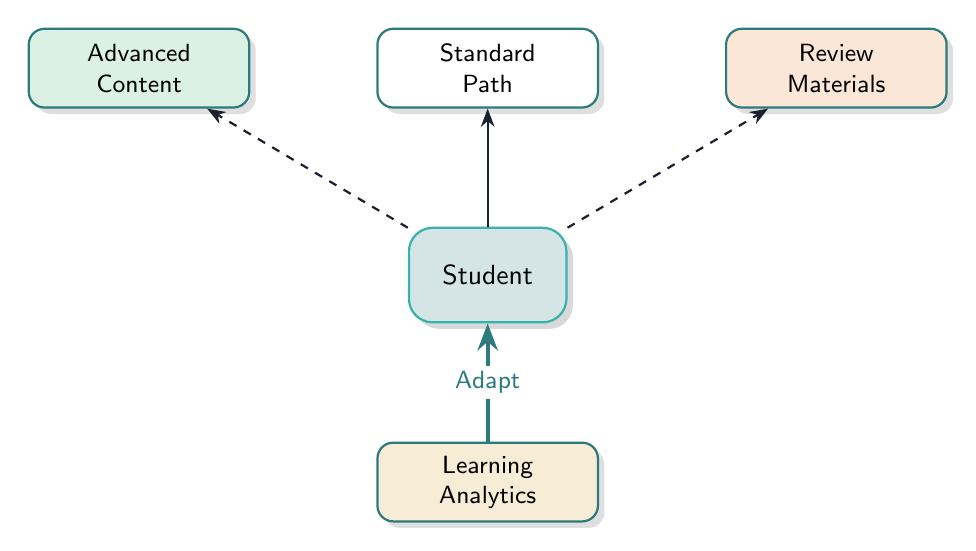
\begin{tikzpicture}[node distance=2cm]
    % Student at center
    \node[basic, fill=shikscolPrimary!20, minimum width=2cm] (student) {Student};
    
    % Learning path nodes
    \node[service, above left=1.5cm and 2cm of student, fill=successGreen!20] (high) {Advanced\\Content};
    \node[service, above=1.5cm of student] (normal) {Standard\\Path};
    \node[service, above right=1.5cm and 2cm of student, fill=warningOrange!20] (review) {Review\\Materials};
    
    % Analytics engine
    \node[service, below=1.5cm of student, fill=shikscolAccent!20] (analytics) {Learning\\Analytics};
    
    % Arrows
    \draw[arrow, dashed] (student) -- (high);
    \draw[arrow] (student) -- (normal);
    \draw[arrow, dashed] (student) -- (review);
    \draw[bigarrow] (analytics) -- node[label] {Adapt} (student);
\end{tikzpicture}
\caption{Adaptive Learning Path Selection}
\end{figure}

\subsection{Learning Analytics}

Teachers receive insights powered by machine learning:

\begin{itemize}
    \item Which lessons cause the most students to rewatch content multiple times?
    \item What quiz questions have the lowest success rates (indicating unclear teaching)?
    \item Which students are at risk of falling behind based on engagement patterns?
    \item How does student performance correlate with time-of-day or day-of-week?
\end{itemize}

These insights drive continuous course improvement.

\section{Collaborative Features}

\subsection{Discussion Forums}

Each course includes threaded discussion boards where:

\begin{itemize}
    \item Students ask questions and help each other
    \item Teachers can mark official answers
    \item The AI assistant can suggest relevant past discussions when students ask questions
    \item Participation contributes to student engagement scores
\end{itemize}

\subsection{Study Groups}

Students can form virtual study groups within a course:

\begin{itemize}
    \item Shared notes and flashcard decks
    \item Group video calls (integrated with WebRTC)
    \item Collaborative whiteboards for working through problems together
    \item Scheduled study sessions with calendar integration
\end{itemize}

\subsection{Peer Review}

For essay assignments and projects, teachers can enable peer review:

\begin{enumerate}
    \item Students submit their work by a deadline
    \item The system randomly assigns each student 3 peers' submissions to review
    \item Students provide feedback using a rubric
    \item Teachers review the peer feedback and assign final grades
\end{enumerate}

This teaches critical thinking and evaluation skills while lightening the teacher's grading burden.

% PART III: FUTURE
%\part{Future Roadmap}

\chapter{Short-Term Enhancements (6-12 Months)}

\section{Mobile Application}

Building native iOS and Android apps using React Native to provide:

\begin{itemize}
    \item Offline video playback (download lectures for viewing without internet)
    \item Push notifications for assignment reminders and grade releases
    \item Biometric authentication (Face ID, fingerprint)
    \item Optimized UI for smaller screens
\end{itemize}

\section{Enhanced Analytics Dashboard}

Expanding the instructor analytics with:

\begin{itemize}
    \item \textbf{Predictive Analytics:} Machine learning models that predict which students are likely to drop out based on engagement patterns, allowing early intervention
    \item \textbf{Comparative Analysis:} Show how current course performance compares to previous semesters
    \item \textbf{Content Effectiveness:} Heat maps showing which video segments students rewatch most, indicating areas of confusion
\end{itemize}

\section{Automated Content Generation}

Using AI to assist teachers with course creation:

\begin{itemize}
    \item Generate quiz questions automatically from lecture transcripts
    \item Create summary flashcards for each lesson
    \item Suggest structure and pacing for new courses based on similar successful courses
\end{itemize}

\section{Accessibility Improvements}

Making education truly inclusive:

\begin{itemize}
    \item Automatic caption generation in multiple languages
    \item Audio descriptions for visual content (for visually impaired students)
    \item Screen reader optimization throughout the platform
    \item High-contrast themes for users with visual impairments
    \item Keyboard navigation for all features
\end{itemize}

\chapter{Medium-Term Innovations (1-2 Years)}

\section{Virtual Labs \& Simulations}

For STEM courses, integrate interactive simulations:

\begin{itemize}
    \item \textbf{Physics Labs:} Simulate projectile motion, electricity circuits, or optics experiments in a virtual environment
    \item \textbf{Chemistry Labs:} Mix virtual chemicals and observe reactions without physical lab access
    \item \textbf{Programming Sandboxes:} Embedded code editors where students write and execute code directly in lessons, with automated test case verification
\end{itemize}

\section{Live Virtual Classrooms}

Real-time video conferencing optimized for education:

\begin{itemize}
    \item Integrated whiteboard with math equation support
    \item Screen sharing with annotation tools
    \item Breakout rooms for small group activities
    \item Recording and automatic transcription for students who miss live sessions
    \item Polls and quizzes during live sessions to check understanding
\end{itemize}

\section{Blockchain Certificates}

Issue tamper-proof credentials:

\begin{itemize}
    \item Course completion certificates stored on a blockchain
    \item Students own their credentials, which can be verified by employers instantly
    \item Micro-credentials for completing individual modules or skill pathways
    \item Stackable credentials that combine into larger certifications or degrees
\end{itemize}

\begin{figure}[H]
\centering
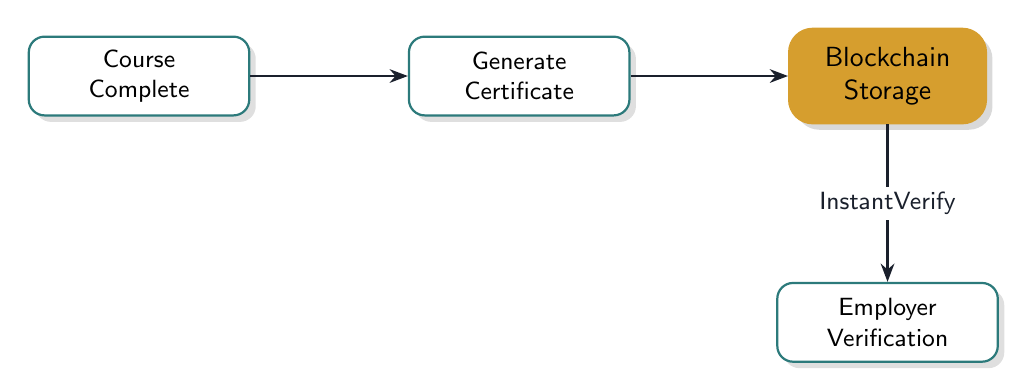
\begin{tikzpicture}[node distance=2cm]
    % Certificate generation
    \node[service] (complete) {Course\\Complete};
    \node[service, right=of complete] (generate) {Generate\\Certificate};
    \node[basic, fill=shikscolAccent, draw=shikscolAccent, right=of generate, minimum width=2.5cm] 
        (blockchain) {Blockchain\\Storage};
    
    % Verification path
    \node[service, below=of blockchain] (verify) {Employer\\Verification};
    
    % Arrows
    \draw[arrow] (complete) -- (generate);
    \draw[arrow] (generate) -- (blockchain);
    \draw[arrow] (blockchain) -- node[label] {Instant\\Verify} (verify);
\end{tikzpicture}
\caption{Blockchain-Based Credential System}
\end{figure}

\section{Advanced AI Tutoring}

Enhancing the AI assistant's capabilities:

\begin{itemize}
    \item \textbf{Conversational Tutoring:} Enable back-and-forth dialogue where the AI guides students through problem-solving step-by-step
    \item \textbf{Voice Interaction:} Students can speak their questions naturally using speech-to-text
    \item \textbf{Multimodal Understanding:} Students can upload screenshots of problems they're stuck on, and the AI analyzes the image and provides help
\end{itemize}

\section{Institutional Integration}

Building connectors for existing educational tools:

\begin{itemize}
    \item Single Sign-On (SSO) with university identity systems (SAML, OAuth)
    \item Grade book export to systems like Banner, PeopleSoft
    \item Calendar integration with Google Calendar, Outlook
    \item Library integration for embedding licensed educational resources
\end{itemize}

\chapter{Long-Term Vision (3-5 Years)}

\section{Personalized AI Agents}

Moving beyond a shared AI assistant to personalized learning companions. Each student would have an AI agent that:

\begin{itemize}
    \item Learns their specific learning style (visual vs. textual, fast vs. methodical pacing)
    \item Maintains long-term memory of what the student knows across all courses
    \item Proactively suggests content when detecting knowledge gaps
    \item Adapts explanations to the student's background and prior knowledge
\end{itemize}

\section{VR/AR Immersive Learning}

Leveraging virtual and augmented reality for experiential education:

\begin{itemize}
    \item \textbf{Historical Immersion:} Walk through ancient Rome while learning about Roman Empire history
    \item \textbf{Medical Training:} Practice surgical procedures in a risk-free VR environment
    \item \textbf{Architecture Visualization:} Design buildings in CAD software and walk through them in VR
    \item \textbf{Language Learning:} Immerse yourself in a virtual Japanese marketplace, practicing conversations with AI-powered NPCs
\end{itemize}

\section{Federated Learning for Privacy}

Implementing machine learning that preserves student privacy. Federated learning allows models to train locally on each student's device, learning from behavior patterns without ever sending raw data to the cloud. Only model updates are shared and aggregated.

This enables highly personalized experiences while maintaining GDPR and FERPA compliance.

\section{Global Education Network}

Creating a marketplace where educators worldwide can collaborate:

\begin{itemize}
    \item Cross-institutional course bundles (take Biology at University A, Chemistry at University B)
    \item Content licensing (University A licenses University B's excellent Machine Learning course)
    \item Shared certification standards recognized across institutions
    \item Translation services enabling courses to be taught in any language automatically
\end{itemize}

\section{Neurofeedback Integration}

Integrating biometric data to optimize learning. Using consumer EEG headbands or smartwatches, the system could detect:

\begin{itemize}
    \item When students are confused or frustrated (adjust pacing or provide hints)
    \item When attention is waning (suggest a break)
    \item Optimal times of day for each student's learning based on cognitive performance patterns
    \item Stress levels during exams (provide calming exercises)
\end{itemize}

\begin{figure}[H]
\centering
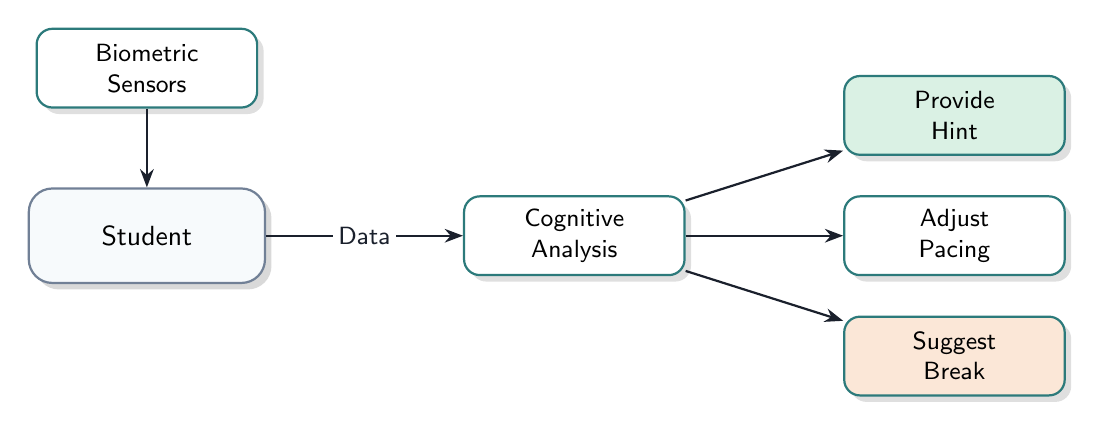
\begin{tikzpicture}[node distance=2.5cm]
    % Student with biometrics
    \node[basic, fill=shikscolLight, draw=shikscolGray] (student) {Student};
    \node[service, above=1cm of student] (bio) {Biometric\\Sensors};
    
    % Analysis
    \node[service, right=2.5cm of student] (analyze) {Cognitive\\Analysis};
    
    % Adaptations
    \node[service, above right=0.5cm and 2cm of analyze, fill=successGreen!20] (hint) {Provide\\Hint};
    \node[service, right=2cm of analyze] (adjust) {Adjust\\Pacing};
    \node[service, below right=0.5cm and 2cm of analyze, fill=warningOrange!20] (break) {Suggest\\Break};
    
    % Arrows
    \draw[arrow] (bio) -- (student);
    \draw[arrow] (student) -- node[label] {Data} (analyze);
    \draw[arrow] (analyze) -- (hint);
    \draw[arrow] (analyze) -- (adjust);
    \draw[arrow] (analyze) -- (break);
\end{tikzpicture}
\caption{Neurofeedback-Driven Learning Optimization}
\end{figure}

\chapter{Conclusion}

\section{The Path Forward}

Shikshak is more than a platform—it's a vision for what education can become when we thoughtfully apply cutting-edge technology to age-old challenges. Every architectural decision, every line of code, and every feature is guided by a simple question: \textit{Does this help students learn better and teachers teach more effectively?}

The microservices architecture ensures Shikshak can scale from a small university pilot program to serving millions of learners globally without a complete rewrite. The AI-first approach ensures students always have support, regardless of time zones or instructor availability. The proctoring system restores trust in online credentials while respecting privacy.

\section{Open Challenges}

We acknowledge that perfect systems don't exist. Shikshak faces ongoing challenges:

\begin{itemize}
    \item \textbf{AI Bias:} Ensuring language models don't perpetuate societal biases in their explanations
    \item \textbf{Access Inequality:} Students without reliable internet or modern devices may struggle with features like AI proctoring
    \item \textbf{Teacher Adaptation:} Many educators are skeptical of AI in education; we must prove value without threatening their role
    \item \textbf{Continuous Improvement:} Education evolves, technology evolves—Shikshak must evolve with them
\end{itemize}

\section{Impact Potential}

If successful, Shikshak could:

\begin{itemize}
    \item Enable universities to offer high-quality online degrees at scale, expanding access to higher education
    \item Reduce teacher burnout by automating routine tasks, letting them focus on authentic human connection and mentorship
    \item Democratize elite education by making expert-created courses available globally at low cost
    \item Provide lifelong learning pathways as careers increasingly require continuous skill updates
    \item Generate datasets that advance learning science, revealing how humans acquire knowledge most effectively
\end{itemize}

\vspace{1cm}

\begin{center}
\large\sffamily\color{shikscolPrimary}
\textit{Education is the great equalizer.}\\[0.3cm]
\normalsize
Technology like Shikshak has the potential to make high-quality learning\\
accessible to anyone with an internet connection, regardless of geography,\\
economic status, or institutional affiliation.
\end{center}

\vspace{1cm}

\begin{center}
\Large\sffamily\bfseries\color{shikscolDark}
The future of education is intelligent, scalable, and deeply human.\\[0.5cm]
\large
Shikshak is building that future, one microservice at a time.
\end{center}

\vfill

\begin{center}

\begin{tikzpicture}
    \draw[shikscolPrimary, line width=2pt] (0,0) -- (12,0);
\end{tikzpicture}
\end{center}

\end{document}
